\documentclass[a4paper,12pt]{article}
\usepackage[utf8]{inputenc}
\usepackage{graphicx}
\usepackage{geometry}
\usepackage{listings}
\usepackage{float}
\usepackage{amsmath}


% Configurazione margini
\usepackage[a4paper, top=3cm, bottom=3cm, left=2.5cm, right=2.5cm]{geometry}


% Configurazione codice SQL
\usepackage{listings}
\usepackage{xcolor}

% Configurazione listings per SQL
\lstdefinelanguage{SQL}{
    keywords={SELECT, FROM, WHERE, ALTER, ADD, CONSTRAINT, CHECK, FOREIGN, KEY, REFERENCES, CREATE, TABLE, PRIMARY},
    % keywordstyle=\color{blue}\bfseries,
    commentstyle=\color{gray}\itshape,
    % stringstyle=\color{red},
    identifierstyle=\color{black},
    basicstyle=\ttfamily\footnotesize,
    morecomment=[l]{--},     % Commenti con --
    morestring=[b]',         % Stringhe delimitate da '
    morestring=[b]"          % Stringhe delimitate da "
}

\lstset{
    showstringspaces=false,
    language=SQL,
    basicstyle=\ttfamily\footnotesize,
    %keywordstyle=\color{blue},
    %stringstyle=\color{red},
    commentstyle=\color{gray},
    frame=single,
    breaklines=true,
    tabsize=2
}


\begin{document}

% Copertina
\begin{titlepage}
    \begin{center}
        % Titolo
        \Large
        \textbf{Elaborato di Basi di Dati} \\
        \vspace{0.5cm}
        \Huge
        \textit{``Artemis Cartesio''} \\
    
        \vspace{2cm}
    
        % Logo
        % Loghi affiancati
        \begin{minipage}{0.4\textwidth}
            \centering
            
\includegraphics[width=\textwidth]{Media/logo_unina.png}
        \end{minipage}
        \hfill
        \begin{minipage}{0.4\textwidth}
            \centering
            
\includegraphics[width=\textwidth]{Media/logo_g.png}
        \end{minipage}
        
        \vspace{2cm}
    
        % Informazioni
        % Informazioni allineate con tabular
        \Large
        \begin{tabular}{l l}
            \textbf{Professore:} & Vincenzo Moscato \\\\
            \textbf{Autori:} & Alessandro Cioffi \hfill N46006940 \\
                             & Antonio Cirino \hfill N46006930 \\
        \end{tabular}
    
        \vfill
    
        \textbf{a.a. 2024/2025}
    \end{center}
\end{titlepage}


% Indice
\newpage
\tableofcontents

% Capitoli
\newpage
\begin{titlepage}
    \begin{center}
        % Titolo
        \Large
        \textbf{Elaborato di Basi di Dati} \\
        \vspace{0.5cm}
        \Huge
        \textit{``nome progetto''} \\
    
        \vspace{2cm}
    
        % Logo
        
\includegraphics[width=0.3\textwidth]{Media/logo_unina.png} \\ 
    
        \vspace{2cm}
    
        % Informazioni
        % Informazioni allineate con tabular
        \Large
        \begin{tabular}{l l}
            \textbf{Professore:} & Vincenzo Moscato \\\\
            \textbf{Autori:} & Alessandro Cioffi \hfill N46006940 \\
                             & Antonio Cirino \hfill N46006930 \\
        \end{tabular}
    
        \vfill
    
        \textbf{a.a. 2024/2025}
    \end{center}
\end{titlepage}

\newpage
\documentclass{article}
\usepackage{graphicx}

\begin{document}

\section{Introduzione}


...

\subsection{Progettazione Concettuale}

...

\subsubsection{Modello E/R portante}

...

\includegraphics[width=\textwidth]{Media/schema_portante.png}

\subsubsection{Modello E/R completo}

...
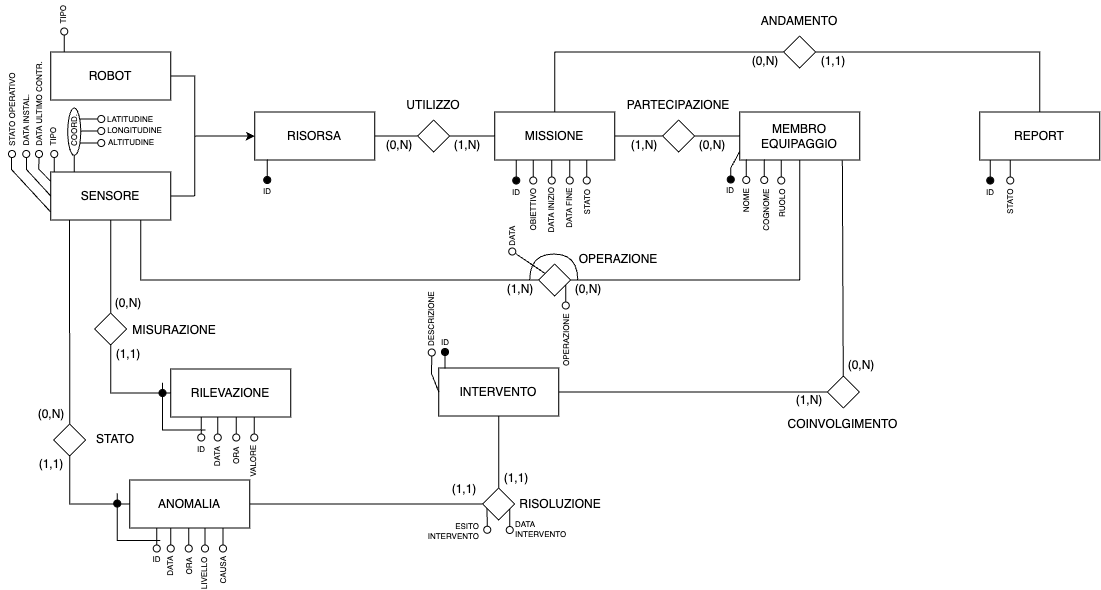
\includegraphics[width=\textwidth]{Media/ER_Completo.png}

\subsection{Progettazione Logica}

La progettazione logica si articola in due fasi:

\begin{enumerate}
    \item \textbf{Trasformazione}: in questa fase, vengono rimossi tutti i costrutti del modello Entità/Relazione (E/R) che non sono direttamente traducibili nel modello logico, come gli attributi composti e gli attributi multi-valore. Gli attributi multi-valore vengono associati direttamente all’entità di partenza, mentre gli attributi composti vengono scomposti nei loro componenti e, se necessario, trasferiti a una nuova entità collegata all’entità originale.
    \item \textbf{Traduzione}: lo schema risultante dalla trasformazione viene convertito nel modello logico attraverso un insieme di regole predeterminate, che possono essere implementate anche tramite strumenti automatizzati. Questa fase non considera direttamente la semantica dei dati, ma si concentra sulla loro struttura.
\end{enumerate}

\subsubsection{Trasformazione}

Durante la fase di trasformazione, vengono eliminati tutti gli attributi che non sono direttamente traducibili nel modello logico. Di seguito vengono descritti i casi specifici presenti nello schema:

\begin{itemize}
    \item \textbf{Attributi multi-valore}: non sono presenti in questo caso, quindi non si rende necessaria alcuna operazione di trasformazione relativa a questa tipologia di attributi.
    \item \textbf{Attributi composti}: l'unico attributo composto identificato è \textbf{Coordinate}, associato all'entità \textit{SENSORE}. Per conformarsi ai requisiti del modello logico, questo attributo è stato scomposto nei suoi componenti: \textbf{Latitudine}, \textbf{Longitudine} e \textbf{Altitudine}. Tali componenti sono stati direttamente associati all’entità di partenza senza creare una nuova entità.
\end{itemize}

Di seguito è riportato lo schema trasformato per l'entità \textit{SENSORI}:

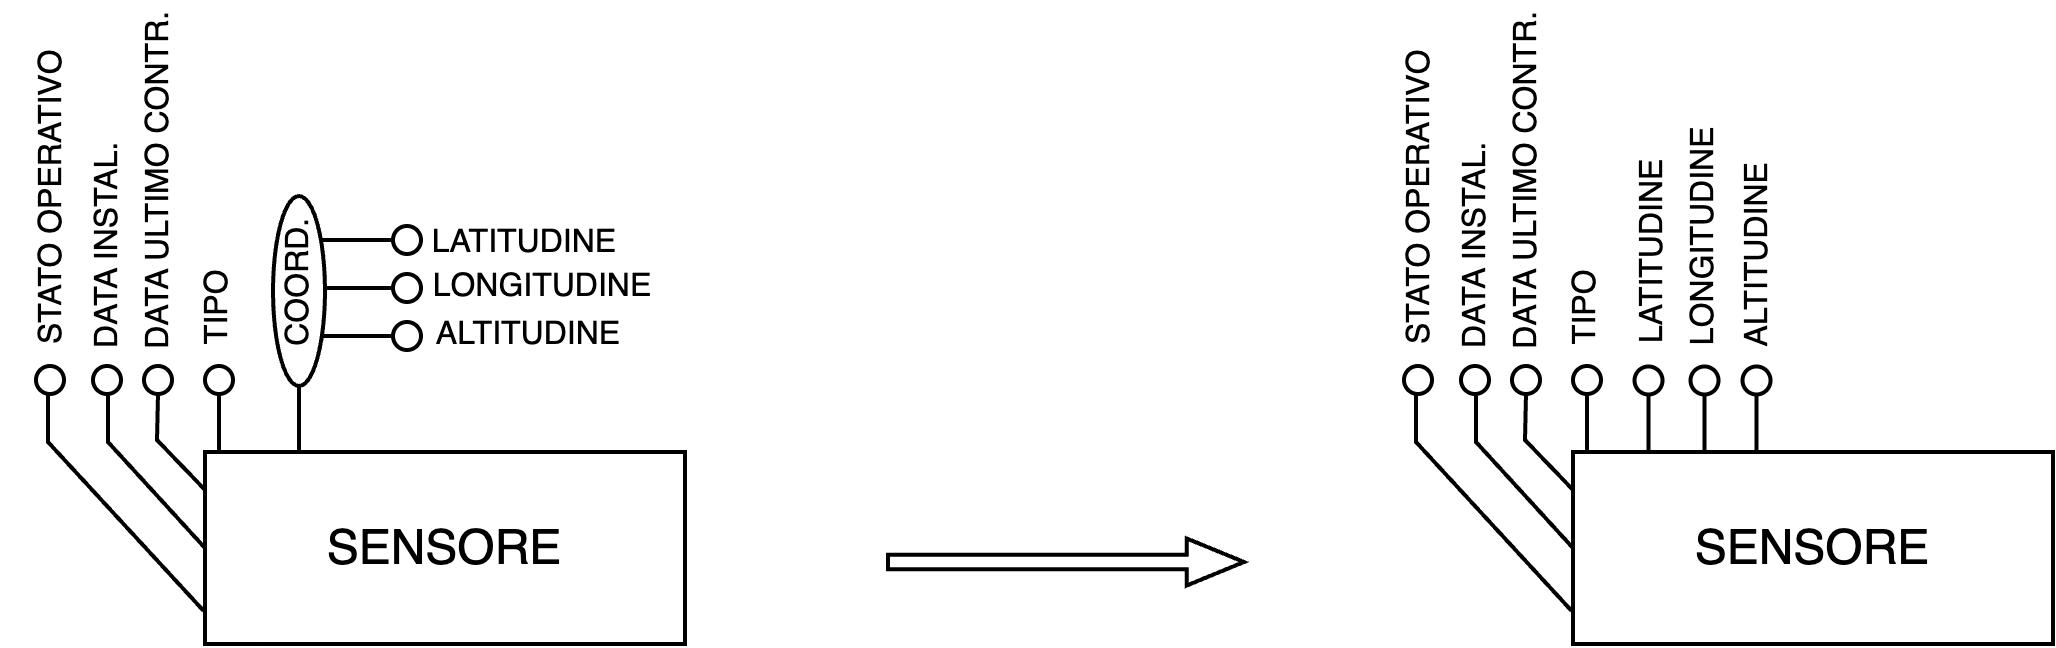
\includegraphics[width=\textwidth]{Media/Trasformazione_Sensore.png}

\textbf{SENSORI} (ID, Data Installazione, Data ultimo controllo, Tipo, \textbf{Latitudine}, \textbf{Longitudine}, \textbf{Altitudine})

\subsubsection{Traduzione}

TODO: DESCRIZIONE FASE TRADUZIONE

\paragraph{Traduzione Entità}

Ogni entità del modello E/R diventa una relazione/tabella.
\begin{itemize}
    \item \textbf{Nome della tabella}: corrisponde al nome dell’entità.
    \item \textbf{Campi della tabella}: corrispondono agli attributi dell’entità.
\end{itemize}

Risultato della Traduzione delle Entità:
\begin{verbatim}
MISSIONI(ID, Obiettivo, Data_Inizio, Data_Fine, Stato);
MEMBI(ID, Nome, Cognome, Ruolo);
REPORT(ID, Stato);
INTERVENTI(ID, Descrizione);
ANOMALIE(ID, Data, Ora, Livello, Causa);
RILEVAZIONI(ID, Data, Ora, Valore);
ROBOT(ID, Tipo);
SENSORI(ID, Data_Installazione, Data_Ultimo_Controllo, Tipo, Stato_Operativo, Latitudine, Longitudine, Altitudine)
\end{verbatim}

\paragraph{Traduzione Relazioni}

\textbf{Specifiche di progettazione}
\begin{itemize}
    \item Per le relazioni N a N ogni associazione diventa una tabella con nome quello dell’associazione al plurale ed ha come campi gli identificatori delle due entità che unisce più gli eventuali attributi dell’associazione stessa. La chiave primaria è data dalla coppia dei due identificatori (che hanno anche un vincolo di integrità referenziale).
    \item Per le relazioni 1 a N agli attributi dell’entità zero si aggiungono quelli dell’entità uno e della relazione (gli attributi della relazione, compreso l’identificatore, vanno nell’entità lato 1). La chiave primaria è quella dell’entità 0 (risparmiamo una tabella, per evitare join a 3 tabelle).
    \item Per le relazioni 1 a 1 ogni associazione diventa una tabella che ha come campi gli identificatori delle entità che correla più gli eventuali attributi. Gli identificatori possono essere entrambi chiavi primarie ma si sceglie quello con cardinalità minore (con partecipazione obbligatoria alla relazione) per evitare valori NULL.
\end{itemize}

\begin{enumerate}
    \item Relazioni \textbf{N a N}
    \begin{itemize}
        \item Ogni associazione N a N diventa una tabella con:
        \begin{itemize}
            \item \textbf{Nome}: corrisponde al nome dell’associazione, al plurale.
            \item \textbf{Campi}: includono gli identificatori delle due entità che collega, più eventuali attributi dell’associazione.
            \item \textbf{Chiave primaria}: composta dalla coppia dei due identificatori.
            \item \textbf{Vincoli di integrità referenziale}: garantiscono la consistenza con le entità collegate.
        \end{itemize}
    \end{itemize}
    \begin{verbatim}
    UTILIZZO_SENSORI (Sensore: Sensori, Missione: Missioni);
    UTILIZZO_ROBOT (Robot: Robot, Missione: Missioni);
    PARTECIPAZIONI (Missione: Missioni, Membro_Equipaggio: Membri_Equipaggio);
    OPERAZIONI (Membro_Equipaggio: Membri_Equipaggio, Sensore: Sensori, Operazione, Data);
    COINVOLGIMENTI (Membro_Equipaggio: Membri_Equipaggio, Intervento: Interventi)
    \end{verbatim}

    \item Relazioni \textbf{1 a N}
    \begin{itemize}
        \item Gli \textbf{attributi dell’entità lato 1} e gli \textbf{attributi della relazione} vengono aggiunti come campi all’entità lato N.
        \item \textbf{Chiave primaria}: rimane quella dell’entità lato N.
        \item Questa scelta consente di ridurre il numero di tabelle, evitando join complessi a 3 tabelle.
    \end{itemize}
    \begin{verbatim}
    REPORT (ID, Stato, Data, Missione: Missioni);
    RILEVAZIONI (ID, Data, Ora, Valore, Sensore: Sensori);
    ANOMALIE (ID, Data, Ora, Livello, Causa, Sensore: Sensori);
    \end{verbatim}

    \item Relazioni \textbf{1 a 1}
    \begin{itemize}
        \item Ogni associazione 1 a 1 diventa una tabella con:
        \begin{itemize}
            \item \textbf{Campi}: includono gli identificatori delle entità che collega, più eventuali attributi.
            \item \textbf{Chiave primaria}: si sceglie l’identificatore dell’entità con cardinalità minima e partecipazione obbligatoria, per evitare valori NULL.
        \end{itemize}
    \end{itemize}
    \begin{verbatim}
    RISOLUZIONI (Intervento: Interventi, Anomalia: Anomalie, Esito_Intervento, Data_Intervento)
    \end{verbatim}
\end{enumerate}

\subsubsection{Modello E/R avanzato}

Le gerarchie di generalizzazione/specializzazione non possono essere direttamente rappresentate nel modello logico relazionale, poiché quest'ultimo non prevede un costrutto equivalente. Per superare questa limitazione, il modello E/R è stato esteso con l'introduzione del costrutto di \textbf{generalizzazione/specializzazione}.

Il costrutto di generalizzazione può essere trasformato in schemi traducibili nel modello logico seguendo tre modalità principali.

\paragraph{Scelta Progettuale}
Per questo progetto è stata adottata la modalità di \textbf{accorpamento della superclasse nelle sottoclassi}:
\begin{itemize}
    \item \textbf{Eliminazione dell’entità padre}: l'entità padre (superclasse) viene eliminata dallo schema.
    \item \textbf{Eredità degli attributi e delle relazioni}: grazie alla proprietà dell’eredità, gli attributi, l’identificatore e le relazioni a cui partecipava l’entità padre vengono trasferiti integralmente alle entità figlie (sottoclassi).
\end{itemize}

Di seguito è riportato il risultato dell'accorpamento relativo alla superclasse \textit{RISORSA} e alle sottoclassi \textit{ROBOT} e \textit{SENSORE}

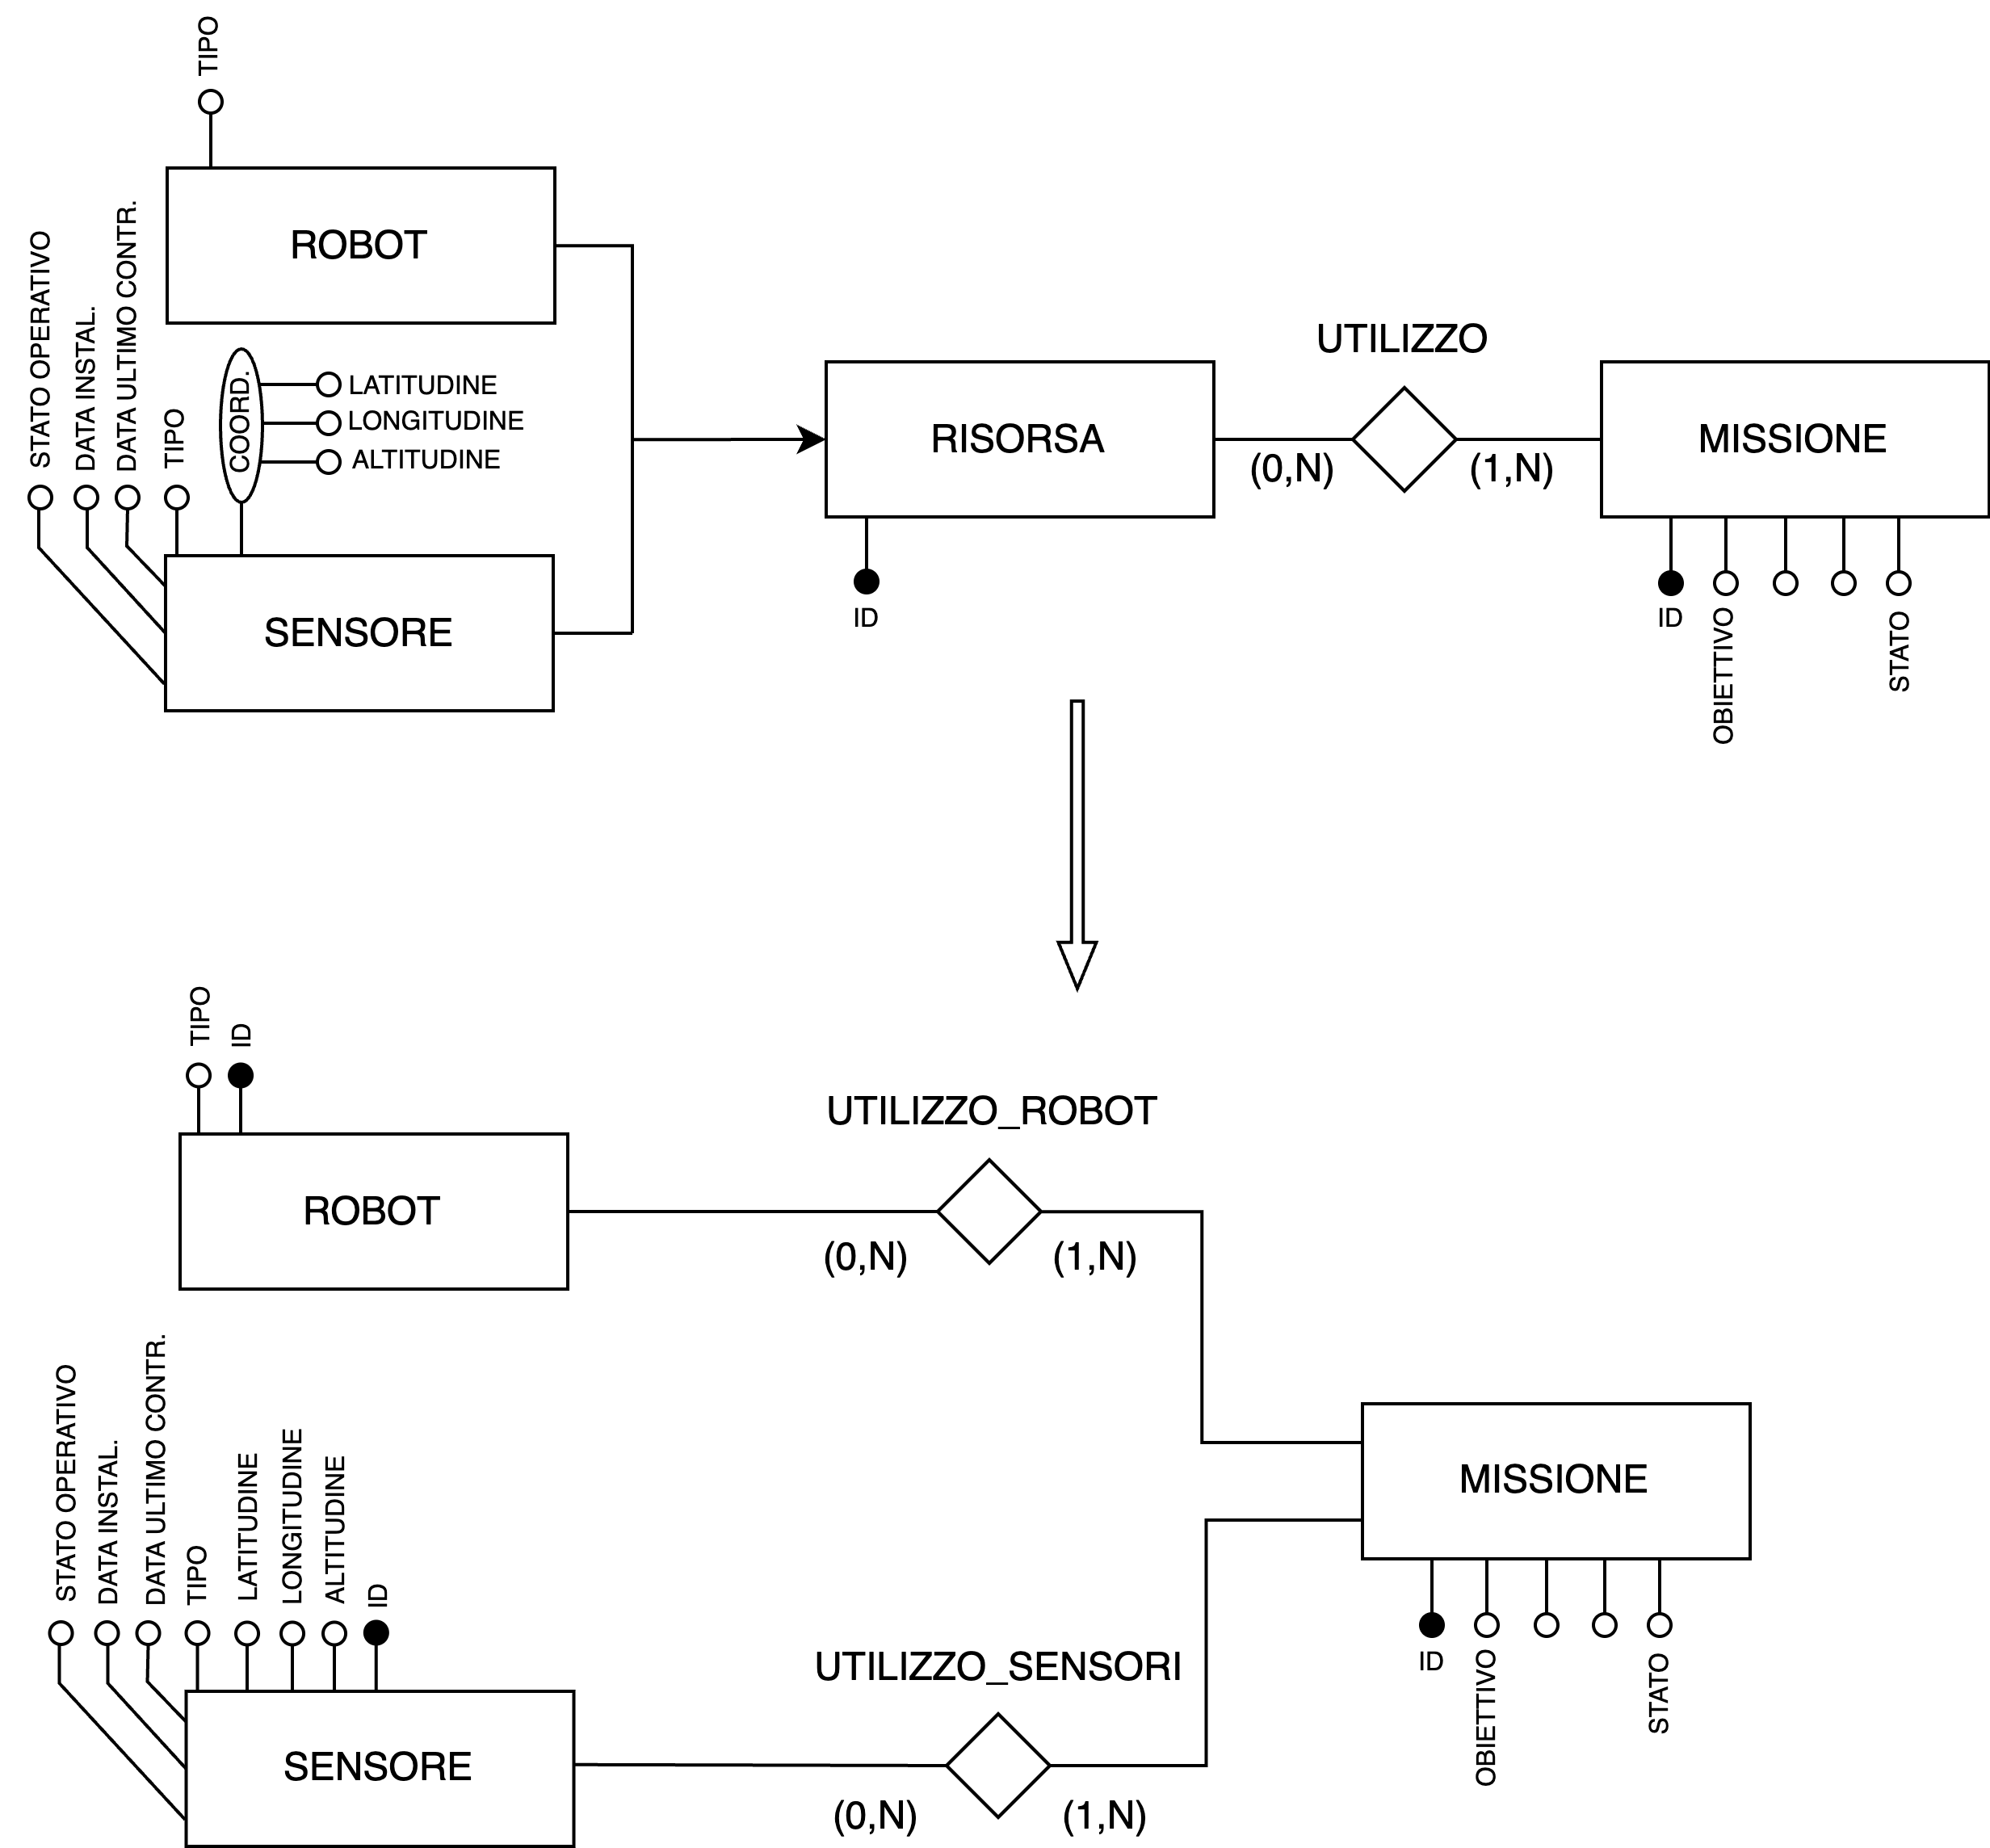
\includegraphics[width=\textwidth]{Media/Generalizzazione_Specializzazione.png}

\subsection{Progettazione Fisica}

I tipi di dato utilizzati per la realizzazione di questo progetto sono:

\begin{itemize}
    \item \textbf{DATE} —> Utilizzato per tutte le date presenti.
    \item \textbf{INTEGER} —> per tutti gli ID che quindi sono formati esclusivamente da numeri e non da lettere;
    \item \textbf{VARCHAR2(N)} —> per tutti gli attributi di tipo testuali, come per esempio nome, cognome, descrizione, ecc..
\end{itemize}

\subsubsection{Tabelle}

\begin{verbatim}
-- Tabella MISSIONI
CREATE TABLE MISSIONI (
    ID INT,
    Obiettivo VARCHAR2(255) NOT NULL,
    Data_Inizio DATE NOT NULL, --NOT NULL o no ?
    Data_Fine DATE,
    Stato VARCHAR2(50) NOT NULL
);

-- Tabella MEMBRI
CREATE TABLE MEMBRI (
    ID INT,
    Nome VARCHAR2(100) NOT NULL,
    Cognome VARCHAR2(100) NOT NULL,
    Ruolo VARCHAR2(100) NOT NULL
);

-- Tabella SENSORI
CREATE TABLE SENSORI (
    ID INT,
    Data_Installazione DATE NOT NULL,
    Data_Ultimo_Controllo DATE,
    Tipo VARCHAR2(100) NOT NULL,
    Latitudine FLOAT NOT NULL,
    Longitudine FLOAT NOT NULL,
    Altitudine FLOAT NOT NULL
);

-- Tabella ROBOT
CREATE TABLE ROBOT (
    ID INT,
    Tipo VARCHAR2(100) NOT NULL
);

-- Tabella ANOMALIE
CREATE TABLE ANOMALIE (
    ID INT,
    Data DATE NOT NULL,
    Ora TIMESTAMP NOT NULL,
    Livello VARCHAR2(50) NOT NULL,
    Causa VARCHAR2(255) NOT NULL,
    Sensori INT
);

-- Tabella INTERVENTI
CREATE TABLE INTERVENTI (
    ID INT,
    Descrizione VARCHAR2(255) NOT NULL
);

-- Tabella RISOLUZIONI
CREATE TABLE RISOLUZIONI (
    Anomalie INT,
    Interventi INT,
    Esito_Intervento VARCHAR2(255),
    Data_Intervento DATE
);

-- Tabella RILEVAZIONI
CREATE TABLE RILEVAZIONI (
    ID INT,
    Data DATE NOT NULL,
    Ora TIMESTAMP NOT NULL,
    Valore FLOAT NOT NULL,
    Sensori INT
);

-- Tabella REPORT
CREATE TABLE REPORT (
    ID INT,
    Stato VARCHAR2(50) NOT NULL,
    Missioni INT
);

-- Tabella UTILIZZO_ROBOT
CREATE TABLE UTILIZZO_ROBOT (
    Robot INT,
    Missioni INT
);

-- Tabella UTILIZZO_SENSORI
CREATE TABLE UTILIZZO_SENSORI (
    Sensori INT,
    Missioni INT
);

-- Tabella COINVOLGIMENTI
CREATE TABLE COINVOLGIMENTI (
    Membri INT,
    Interventi INT
);

-- Tabella OPERAZIONI
CREATE TABLE OPERAZIONI (
    Membri INT,
    Sensori INT,
    Stato_Operativo VARCHAR2(50) NOT NULL,
    Operazione VARCHAR2(255)
);

-- Tabella PARTECIPAZIONI
CREATE TABLE PARTECIPAZIONI (
    Missione INT,
    Membri INT
);

-- Tabella SENSORI_MISSIONI
CREATE TABLE SENSORI_MISSIONI (
    Sensore_ID INT,
    Missione_ID INT,
    PRIMARY KEY (Sensore_ID, Missione_ID),
    FOREIGN KEY (Sensore_ID) REFERENCES SENSORI(ID),
    FOREIGN KEY (Missione_ID) REFERENCES MISSIONI(ID)
);

-- Tabella MEMBRI_MISSIONI
CREATE TABLE MEMBRI_MISSIONI (
    Membro_ID INT,
    Missione_ID INT,
    PRIMARY KEY (Membro_ID, Missione_ID),
    FOREIGN KEY (Membro_ID) REFERENCES MEMBRI(ID),
    FOREIGN KEY (Missione_ID) REFERENCES MISSIONI(ID)
);
\end{verbatim}

\subsubsection{Chiavi primarie}

\begin{verbatim}
--AGGIUNTA CHIAVI PRIMARIE
ALTER TABLE MISSIONI ADD CONSTRAINT PK_MISSIONI PRIMARY KEY (ID);
ALTER TABLE MEMBRI ADD CONSTRAINT PK_MEMBRI PRIMARY KEY (ID);
ALTER TABLE SENSORI ADD CONSTRAINT PK_SENSORI PRIMARY KEY (ID);
ALTER TABLE ROBOT ADD CONSTRAINT PK_ROBOT PRIMARY KEY (ID);
ALTER TABLE ANOMALIE ADD CONSTRAINT PK_ANOMALIE PRIMARY KEY (ID);
ALTER TABLE INTERVENTI ADD CONSTRAINT PK_INTERVENTI PRIMARY KEY (ID);
ALTER TABLE RILEVAZIONI ADD CONSTRAINT PK_RILEVAZIONI PRIMARY KEY (ID);
ALTER TABLE REPORT ADD CONSTRAINT PK_REPORT PRIMARY KEY (ID);
ALTER TABLE RISOLUZIONI ADD CONSTRAINT PK_RISOLUZIONI PRIMARY KEY (Anomalie, Interventi);
ALTER TABLE UTILIZZO_ROBOT ADD CONSTRAINT PK_UTILIZZO_ROBOT PRIMARY KEY (Robot, Missioni);
ALTER TABLE UTILIZZO_SENSORI ADD CONSTRAINT PK_UTILIZZO_SENSORI PRIMARY KEY (Sensori, Missioni);
ALTER TABLE COINVOLGIMENTI ADD CONSTRAINT PK_COINVOLGIMENTI PRIMARY KEY (Membri, Interventi);
ALTER TABLE OPERAZIONI ADD CONSTRAINT PK_OPERAZIONI PRIMARY KEY (Membri, Sensori);
ALTER TABLE PARTECIPAZIONI ADD CONSTRAINT PK_PARTECIPAZIONI PRIMARY KEY (Missione, Membri);
\end{verbatim}

\subsubsection{Chiavi esterne}

\begin{verbatim}
--AGGIUNTE CHIAVI ESTERNE
ALTER TABLE ANOMALIE ADD CONSTRAINT FK_ANOMALIE_SENSORI FOREIGN KEY (Sensori) REFERENCES SENSORI(ID);
ALTER TABLE RISOLUZIONI ADD CONSTRAINT FK_RISOLUZIONI_ANOMALIE FOREIGN KEY (Anomalie) REFERENCES ANOMALIE(ID);
ALTER TABLE RISOLUZIONI ADD CONSTRAINT FK_RISOLUZIONI_INTERVENTI FOREIGN KEY (Interventi) REFERENCES INTERVENTI(ID);
ALTER TABLE RILEVAZIONI ADD CONSTRAINT FK_RILEVAZIONI_SENSORI FOREIGN KEY (Sensori) REFERENCES SENSORI(ID);
ALTER TABLE REPORT ADD CONSTRAINT FK_REPORT_MISSIONI FOREIGN KEY (Missioni) REFERENCES MISSIONI(ID);
ALTER TABLE UTILIZZO_ROBOT ADD CONSTRAINT FK_UTILIZZO_ROBOT_ROBOT FOREIGN KEY (Robot) REFERENCES ROBOT(ID);
ALTER TABLE UTILIZZO_ROBOT ADD CONSTRAINT FK_UTILIZZO_ROBOT_MISSIONI FOREIGN KEY (Missioni) REFERENCES MISSIONI(ID);
ALTER TABLE UTILIZZO_SENSORI ADD CONSTRAINT FK_UTILIZZO_SENSORI_SENSORI FOREIGN KEY (Sensori) REFERENCES SENSORI(ID);
ALTER TABLE UTILIZZO_SENSORI ADD CONSTRAINT FK_UTILIZZO_SENSORI_MISSIONI FOREIGN KEY (Missioni) REFERENCES MISSIONI(ID);
ALTER TABLE COINVOLGIMENTI ADD CONSTRAINT FK_COINVOLGIMENTI_MEMBRI FOREIGN KEY (Membri) REFERENCES MEMBRI(ID);
ALTER TABLE COINVOLGIMENTI ADD CONSTRAINT FK_COINVOLGIMENTI_INTERVENTI FOREIGN KEY (Interventi) REFERENCES INTERVENTI(ID);
ALTER TABLE OPERAZIONI ADD CONSTRAINT FK_OPERAZIONI_MEMBRI FOREIGN KEY (Membri) REFERENCES MEMBRI(ID);
ALTER TABLE OPERAZIONI ADD CONSTRAINT FK_OPERAZIONI_SENSORI FOREIGN KEY (Sensori) REFERENCES SENSORI(ID);
ALTER TABLE PARTECIPAZIONI ADD CONSTRAINT FK_PARTECIPAZIONI_MISSIONE FOREIGN KEY (Missione) REFERENCES MISSIONI(ID);
ALTER TABLE PARTECIPAZIONI ADD CONSTRAINT FK_PARTECIPAZIONI_MEMBRI FOREIGN KEY (Membri) REFERENCES MEMBRI(ID);
\end{verbatim}

\subsubsection{Vincoli di check}

\begin{verbatim}
-- Vincoli per SENSORI
ALTER TABLE SENSORI ADD CONSTRAINT CK_SENSORI_TIPO CHECK (Tipo IN ('Temperatura', 'Pressione', 'Gas', 'Radiazioni', 'Geologia'));

-- Vincoli per OPERAZIONI
ALTER TABLE OPERAZIONI ADD CONSTRAINT CK_OPERAZIONI_STATO CHECK (Stato_Operativo IN ('Attivo', 'Standby', 'Manutenzione', 'Malfunzionante'));

-- Vincoli per ANOMALIE
ALTER TABLE ANOMALIE ADD CONSTRAINT CK_ANOMALIE_LIVELLO CHECK (Livello IN ('Bassa', 'Media', 'Alta', 'Critica'));

-- Vincoli per MISSIONI
ALTER TABLE MISSIONI ADD CONSTRAINT CK_MISSIONI_STATO CHECK (Stato IN ('Pianificata', 'In corso', 'Completata', 'Annullata'));
\end{verbatim}

\end{document}
\newpage
\section{Ottimizzazione DB}

\subsection{Indici}

Un \textbf{indice} in un sistema di gestione di database (DBMS) è una struttura dati organizzata che consente di individuare rapidamente un determinato record all'interno di un file di dati. Uno dei principali vantaggi dell'utilizzo degli indici è il miglioramento delle prestazioni delle query: gli indici permettono di ridurre il tempo necessario per cercare i dati, evitando una scansione completa della tabella.

Creare indici sui campi che vengono frequentemente utilizzati nei filtri delle query (ad esempio, con condizioni \texttt{WHERE}, \texttt{JOIN}, \texttt{ORDER BY} o \texttt{GROUP BY}) può velocizzare significativamente l'elaborazione delle richieste, ottimizzando il sistema nel suo complesso.

Tuttavia, è importante bilanciare l'uso degli indici per evitare costi aggiuntivi durante le operazioni di scrittura come \texttt{INSERT}, \texttt{UPDATE} e \texttt{DELETE}, poiché gli indici devono essere aggiornati ogni volta che i dati della tabella vengono modificati.

Tralasciando gli indici sulla chiave primaria, in quanto il DBMS crea un indice per ogni chiave primaria della tabella, abbiamo pensato di aggiungere questi indici: \\

\begin{lstlisting}
CREATE INDEX idx_missioni_stato ON MISSIONI(Stato); 
-- utile per filtrare missioni sullo stato

CREATE INDEX idx_membri_ruolo ON MEMBRI(Ruolo); 
-- utile per filtrare sul ruolo dei membri

CREATE INDEX idx_robot_tipo ON ROBOT(Tipo); 
-- utile per filtrare sul tipo di robot

CREATE INDEX idx_report_data ON REPORT(Data);

CREATE INDEX idx_rilevazioni_sensori_data ON RILEVAZIONI(Sensori, Data);
\end{lstlisting}

\subsection{Concorrenza}

Per la gestione della concorrenza abbiamo scelto di adottare il protocollo \textbf{2PL stretto}, una variante del \textbf{2PL}. Entrambi i protocolli si basano sul meccanismo del \textbf{lock}, che consente di gestire la concorrenza e garantire la \textbf{serializzabilità delle transazioni}.

Il suo funzionamento prevede:

\begin{itemize}
    \item \texttt{lock()}: ogni oggetto è protetto da un lock;
    \item \texttt{read\_lock()}: se una transazione vuole effettuare una lettura su uno oggetto. Più transazioni possono leggere contemporaneamente lo stesso oggetto (condivisione).
    \item \texttt{write\_lock()}: è esclusivo e consente a una sola transazione di modificare l'oggetto per volta.
    \item \texttt{unlock()}: Ogni lock, una volta terminata l'operazione, deve essere rilasciato (unlock).
\end{itemize}

Gli oggetti possono trovarsi in tre stati: \textbf{libero}, \textbf{bloccato in lettura}, o \textbf{bloccato in scrittura}.

La scelta del \textbf{2PL stretto} rispetto al \textbf{2PL} è dovuta al fatto che il \textbf{2PL stretto} evita l'anomalia delle \textbf{letture sporche} (dirty reads), che possono verificarsi in altri approcci di gestione della concorrenza.

Il 2PL stretto prevede due fasi:

\begin{itemize}
    \item \textbf{fase crescente}: è la fase in cui una transazione acquisisce mediante \texttt{read\_lock} e \texttt{write\_lock} tutte le risorse su cui dovrà effettuare operazioni di lettura e scrittura.
    \item \textbf{fase decrescente}: è la fase in cui attraverso l'\texttt{unlock} si vanno a rilasciare le risorse. In particolare questa fase nel caso di 2PL stretto può essere effettuata solo se la transazione termina con una commit o con un abort.
\end{itemize}

Questo approccio garantisce che le transazioni siano serializzabili, impedendo conflitti e mantenendo la consistenza dei dati.

\subsection{Affidabilità}

Il controllo di \textbf{affidabilità} in un sistema di basi di dati ha come obiettivo principale il \textbf{ripristino} dello stato corretto del sistema (recovery) in seguito a guasti accidentali o intenzionali, che possano compromettere la funzionalità del sistema stesso. I guasti possono essere legati sia a malfunzionamenti hardware (ad esempio, guasti su disco o memoria) che software (ad esempio, crash di applicazioni o errori di sistema).

Il sistema di affidabilità si basa sulla gestione delle \textbf{transazioni}, che sono le unità fondamentali delle operazioni nel database, garantendo \textbf{atomicità} (le transazioni sono eseguite in modo completo o non eseguite affatto) e \textbf{persistenza} (i dati delle transazioni devono essere memorizzati in modo permanente una volta che la transazione è stata completata correttamente).

\subsubsection{Backup}

Per garantire un alto livello di affidabilità, il nostro sistema di database implementa la strategia di backup RAID 1, che offre una soluzione di mirroring. In un sistema RAID 1, ogni dato scritto sul disco primario viene duplicato in tempo reale su un disco secondario, chiamato "mirror". Questa tecnica garantisce che, in caso di guasto di uno dei dischi, i dati siano ancora disponibili sull'altro disco, riducendo il rischio di perdita di informazioni e migliorando la disponibilità del sistema.

\begin{figure}[h]
    \centering
    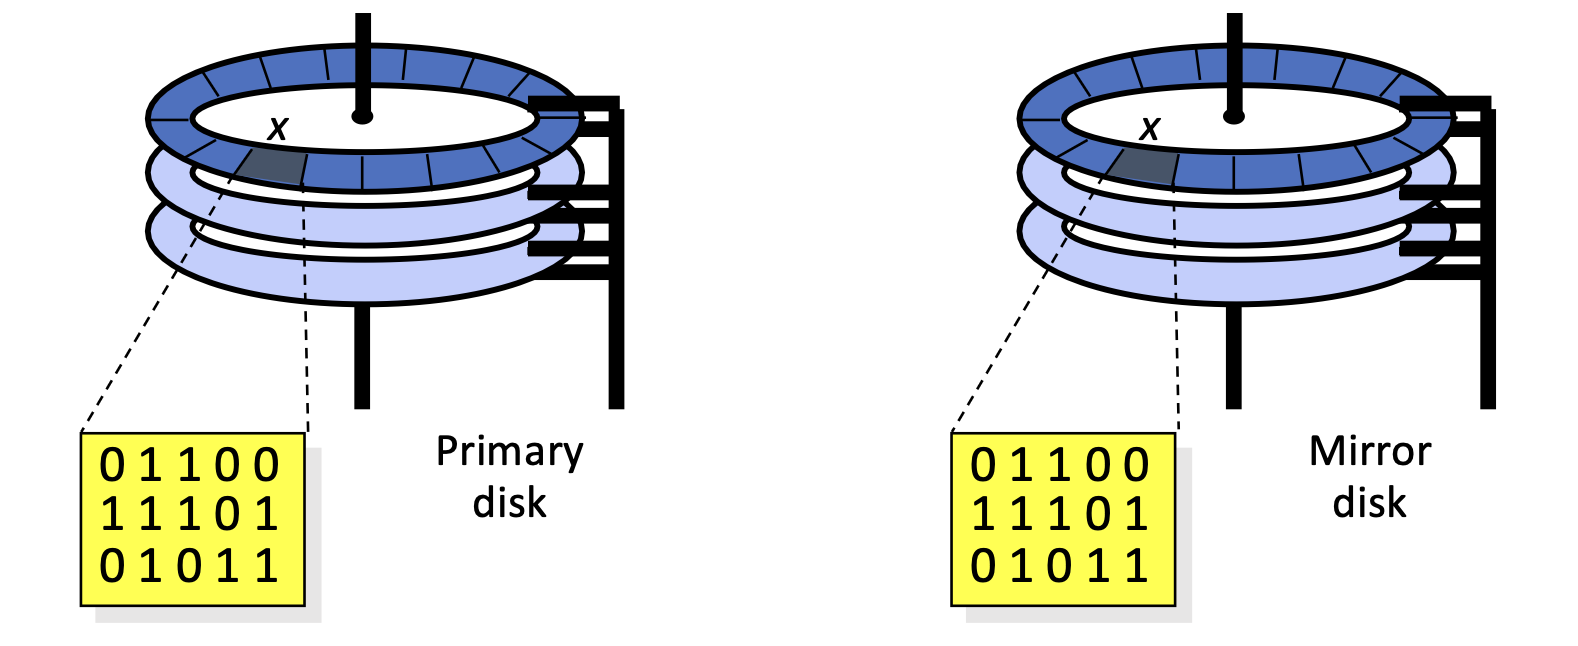
\includegraphics[width=0.5\textwidth]{Media/raid.png}
    \caption{RAID 1 Mirroring}
    \label{fig:raid}
\end{figure}

\subsubsection{Recovery}

Il gestore dell’affidabilità deve gestire l’esecuzione dei comandi transazionali di \texttt{begin transaction}, \texttt{commit}, \texttt{rollback} e tutte le operazioni di ripristino dopo i guasti.

Per poter effettuare ciò, il gestore deve possedere un file di log: un file presente su memoria stabile che registra tutte le operazioni svolte dalle transazioni nel loro ordine di esecuzione.

Il log è quindi una sorta di “diario di bordo” che, in un qualsiasi istante, permette di ricostituire il contenuto corretto della base dei dati a seguito di malfunzionamenti.

\begin{figure}[h]
    \centering
    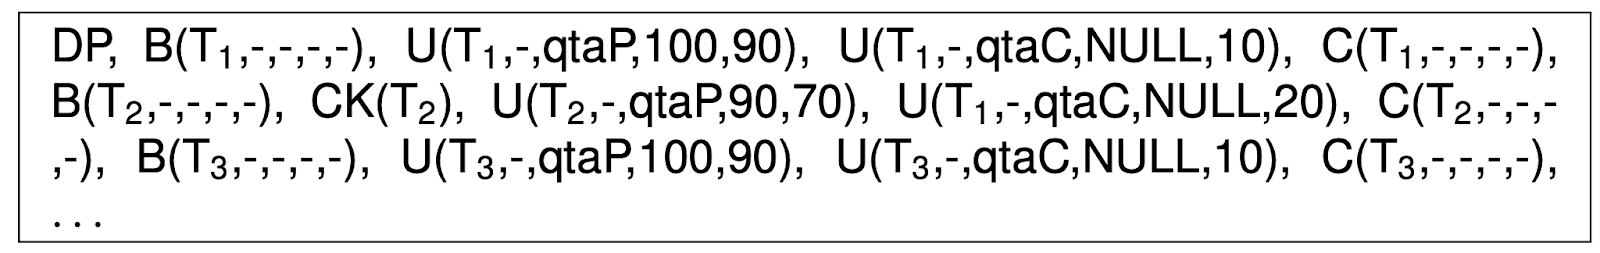
\includegraphics[width=0.8\textwidth]{Media/log.png}
    \caption{File di log}
    \label{fig:log}
\end{figure}

\paragraph{Tecniche di recovery}

\begin{itemize}
    \item \textbf{Ripresa a freddo}: Nel caso di guasti hard sui dispositivi di memoria di massa (es. guasti ai dischi rigidi) si perde sia la memoria centrale che quella secondaria, ma la memoria stabile (come i dispositivi di backup) rimane intatta. In queste situazioni, viene effettuata la ripresa a freddo (cold restart), che richiede un ripristino più approfondito, attingendo ai backup e ai log per recuperare i dati persi.
    \item \textbf{Ripresa a caldo}: Nel caso di guasti soft (es. errori di programma, crash di sistema, caduta di tensione, ecc.) si perde il contenuto della sola memoria centrale (mentre rimangono intatte la memoria secondaria e quella stabile). In tali situazioni, viene effettuata la cosiddetta ripresa a caldo (warm restart).
\end{itemize}

In entrambi i casi, la procedura di ripristino avviene nelle seguenti fasi (modello fail-stop):

\begin{enumerate}
    \item si forza l’arresto completo delle transazioni attive sul sistema di basi di dati;
    \item viene ripristinato il corretto funzionamento del sistema operativo;
    \item viene effettuata la procedura di ripristino.
\end{enumerate}

\newpage
\section{Stored Procedures}

\subsection{Query}

\subsection{Views}

\subsection{Procedures}

\subsection{Triggers}
\newpage
\section{Oracle APEX}

\subsection{Introduzione}
\textbf{Oracle APEX} (Application Express) è una piattaforma di sviluppo applicativo low-code che consente di creare applicazioni web scalabili, sicure e altamente performanti utilizzando il database Oracle come base.\\
Con Oracle APEX, è possibile sfruttare strumenti integrati per la creazione di interfacce utente, la gestione dei dati e la personalizzazione delle funzionalità, rendendo il processo di sviluppo rapido ed efficiente. È particolarmente utile per automatizzare processi aziendali, creare report interattivi e implementare soluzioni personalizzate su misura per le esigenze delle organizzazioni.

\subsection{Home}

\begin{figure}[ht!]
    \centering
    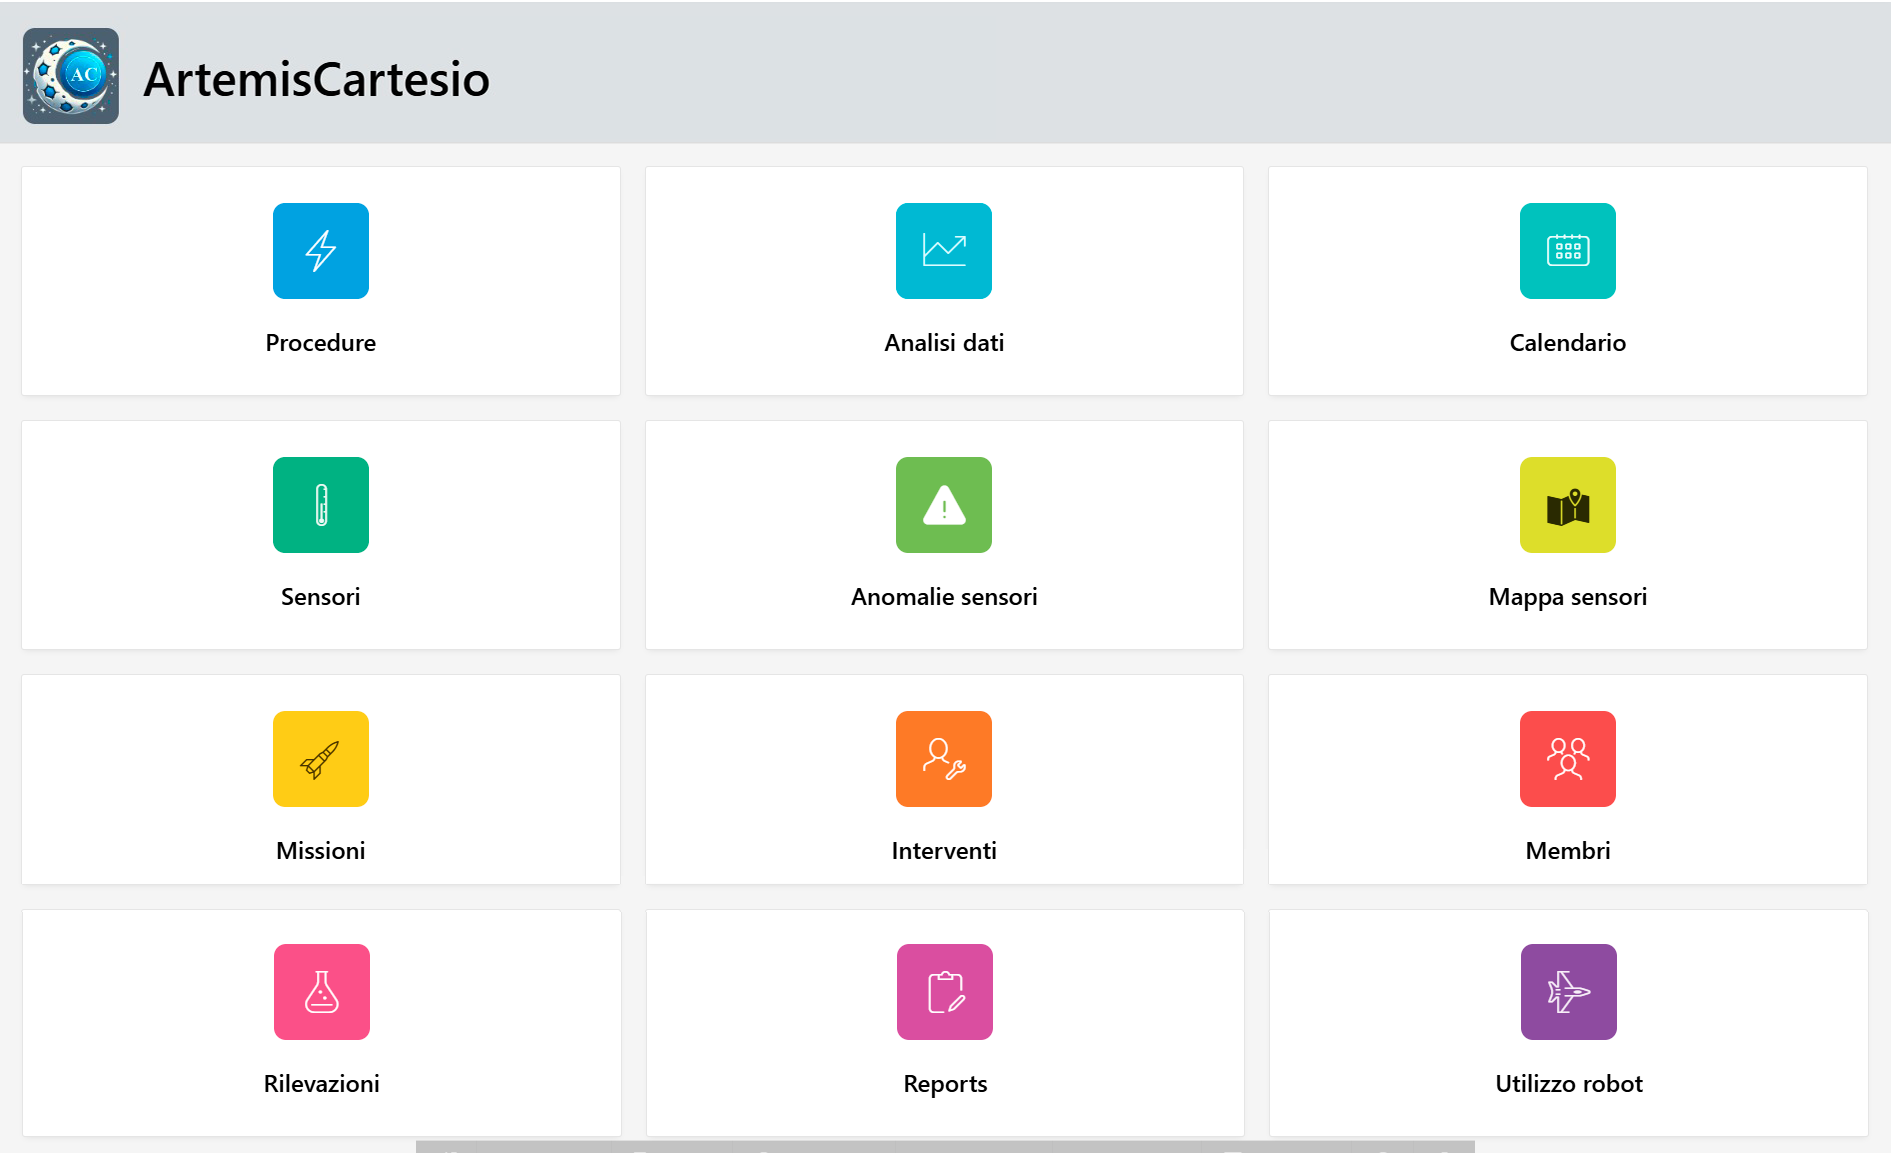
\includegraphics[width=\textwidth]{Media/App/home.png}
    \caption{Home page dell'applicazione}
    \label{fig:home_page}
\end{figure}

\noindent
In figura (Figura~\ref{fig:home_page}) è rappresentata la schermata principale dell'applicazione, progettata per gestire e monitorare ogni aspetto di una missione spaziale. La home page presenta una serie di funzionalità principali, ciascuna accessibile tramite icone intuitive e facilmente identificabili, che semplificano la navigazione e l'interazione con il sistema.\\
L'interfaccia è user-friendly e ben strutturata, progettata per garantire l'efficienza e la facilità d'uso per i membri dell'equipaggio della missione. Grazie all'organizzazione intuitiva, si può accedere rapidamente alle informazioni necessarie e ai moduli specifici per completare i propri compiti.

\subsection{Procedure}
\begin{figure}[ht!]
    \centering
    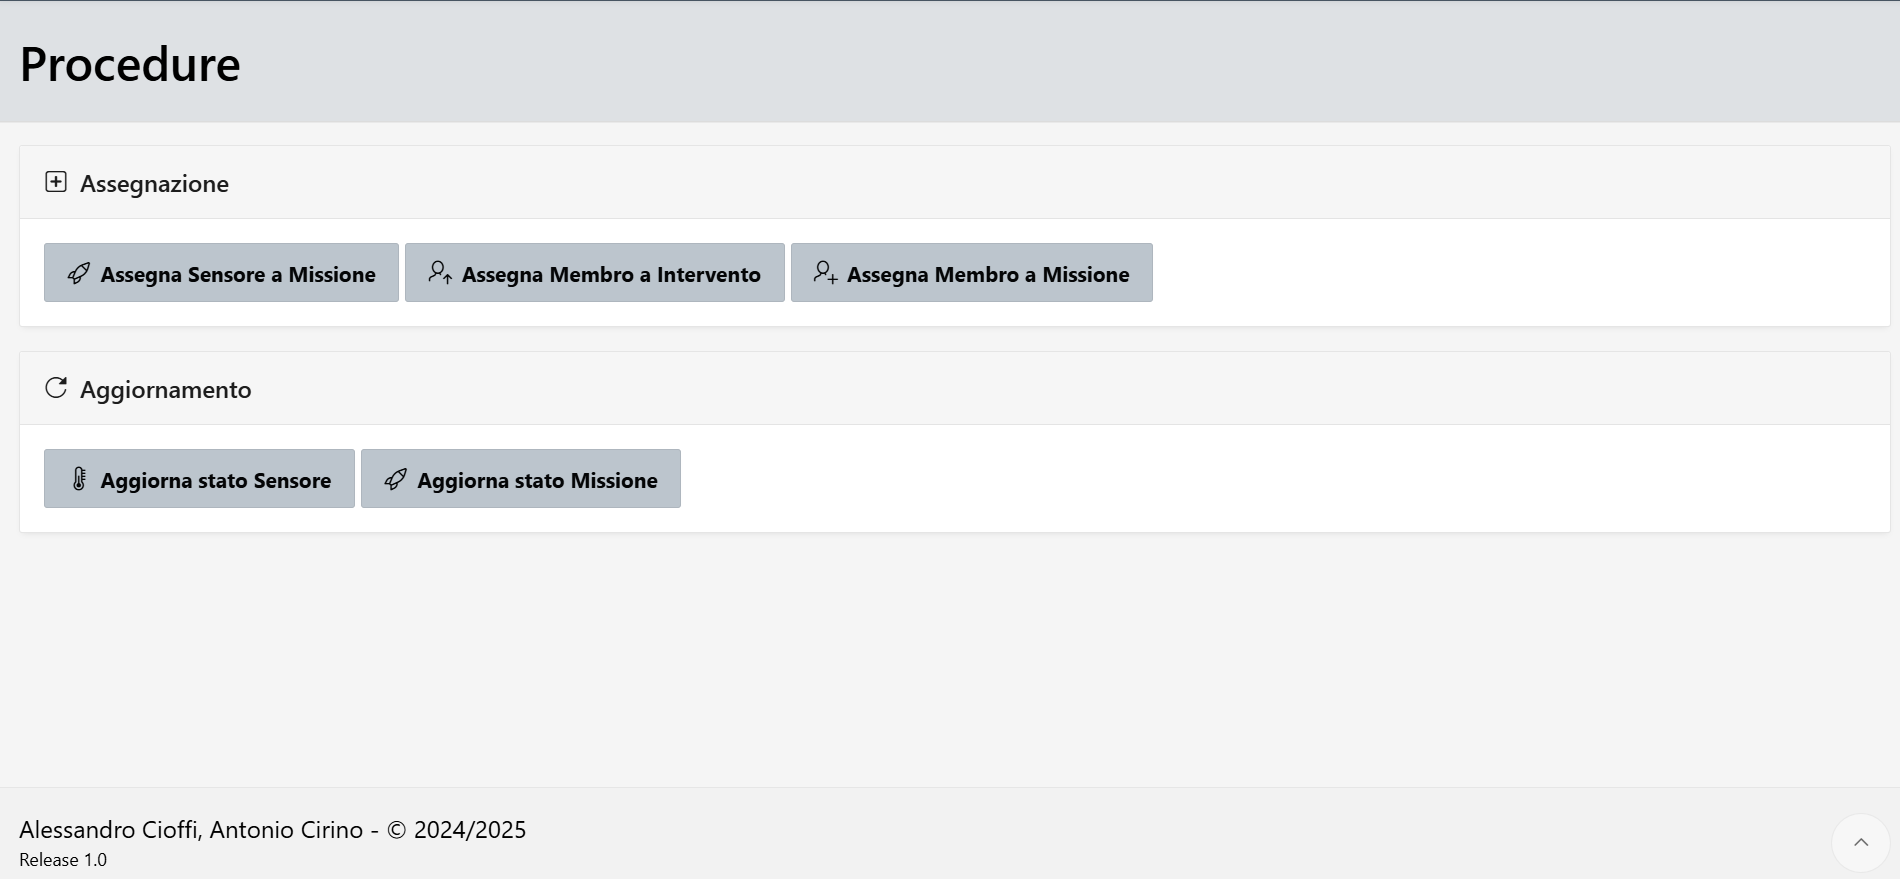
\includegraphics[width=\textwidth]{Media/App/procedure.png}
    \caption{Schermata della sezione \textit{Procedure}}
    \label{fig:procedure}
\end{figure}

\noindent
La schermata \textit{Procedure} è divisa in due sezioni: \textbf{Assegnazione} e \textbf{Aggiornamento}.

\paragraph{Assegnazione} Questa sezione permette di gestire l'allocazione delle risorse e del personale per le varie attività. Le funzionalità principali includono:
\begin{itemize}
    \item \textbf{Assegna Sensore a Missione}: consente di associare specifici sensori a una missione attiva.
    \item \textbf{Assegna Membro a Intervento}: permette di designare un membro del team per un determinato intervento tecnico (Figura~\ref{fig:procedura_assegnazione}).
    \item \textbf{Assegna Membro a Missione}: utilizzato per assegnare personale a una missione specifica.
\end{itemize}
\paragraph{Aggiornamento}
In questa sezione si possono effettuare aggiornamenti sullo stato dei sensori e delle missioni, garantendo che le informazioni siano sempre accurate e aggiornate. Le opzioni includono:
\begin{itemize}
    \item \textbf{Aggiorna stato Sensore}: modifica dello stato operativo di un sensore (attivo, malfunzionante, manutenzione, stand by) e della data dell'ultimo controllo (Figura~\ref{fig:procedura_aggiornamento}).
    \item \textbf{Aggiorna stato Missione}: consente di aggiornare lo stato di avanzamento di una missione (pianificata, in corso, completata, annullata).
\end{itemize}

\begin{figure}[ht!]
    \centering
    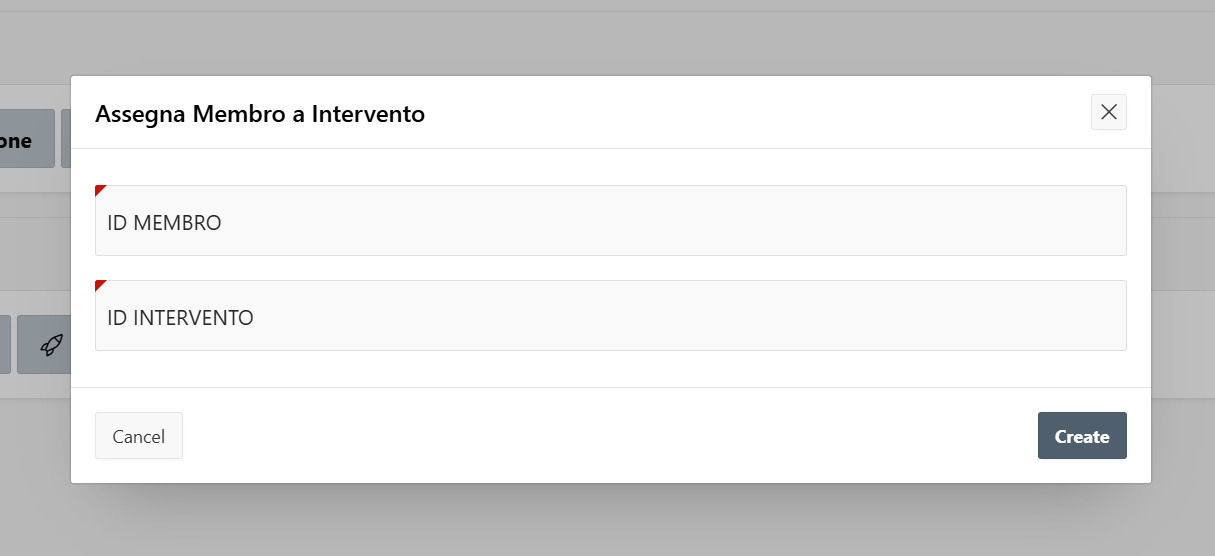
\includegraphics[width=0.8\textwidth]{Media/App/procedure_assegnazione.png}
    \caption{Finestra di dialogo per l'assegnazione di un membro ad un intervento}
    \label{fig:procedura_assegnazione}
\end{figure}

\begin{figure}[ht!]
    \centering
    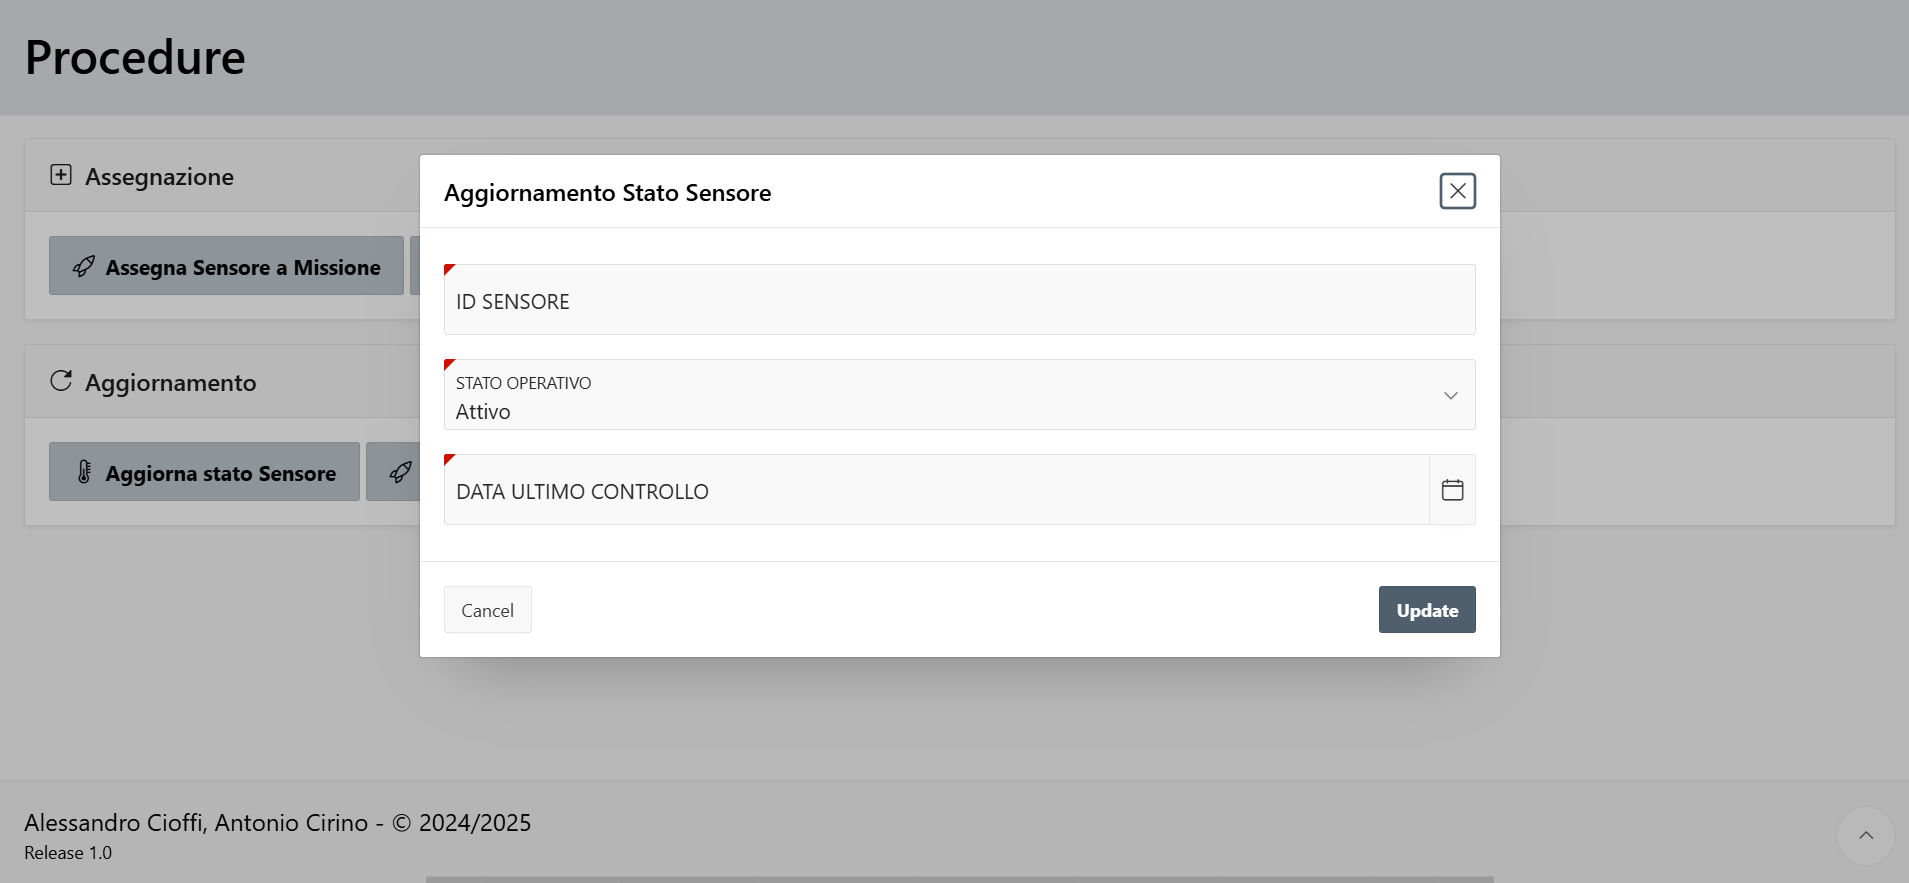
\includegraphics[width=0.8\textwidth]{Media/App/procedure_aggiornamento.png}
    \caption{Finestra di dialogo per l'aggiornamento di un sensore}
    \label{fig:procedura_aggiornamento}
\end{figure}


\subsection{Analisi dati}

\begin{figure}[ht!]
    \centering
    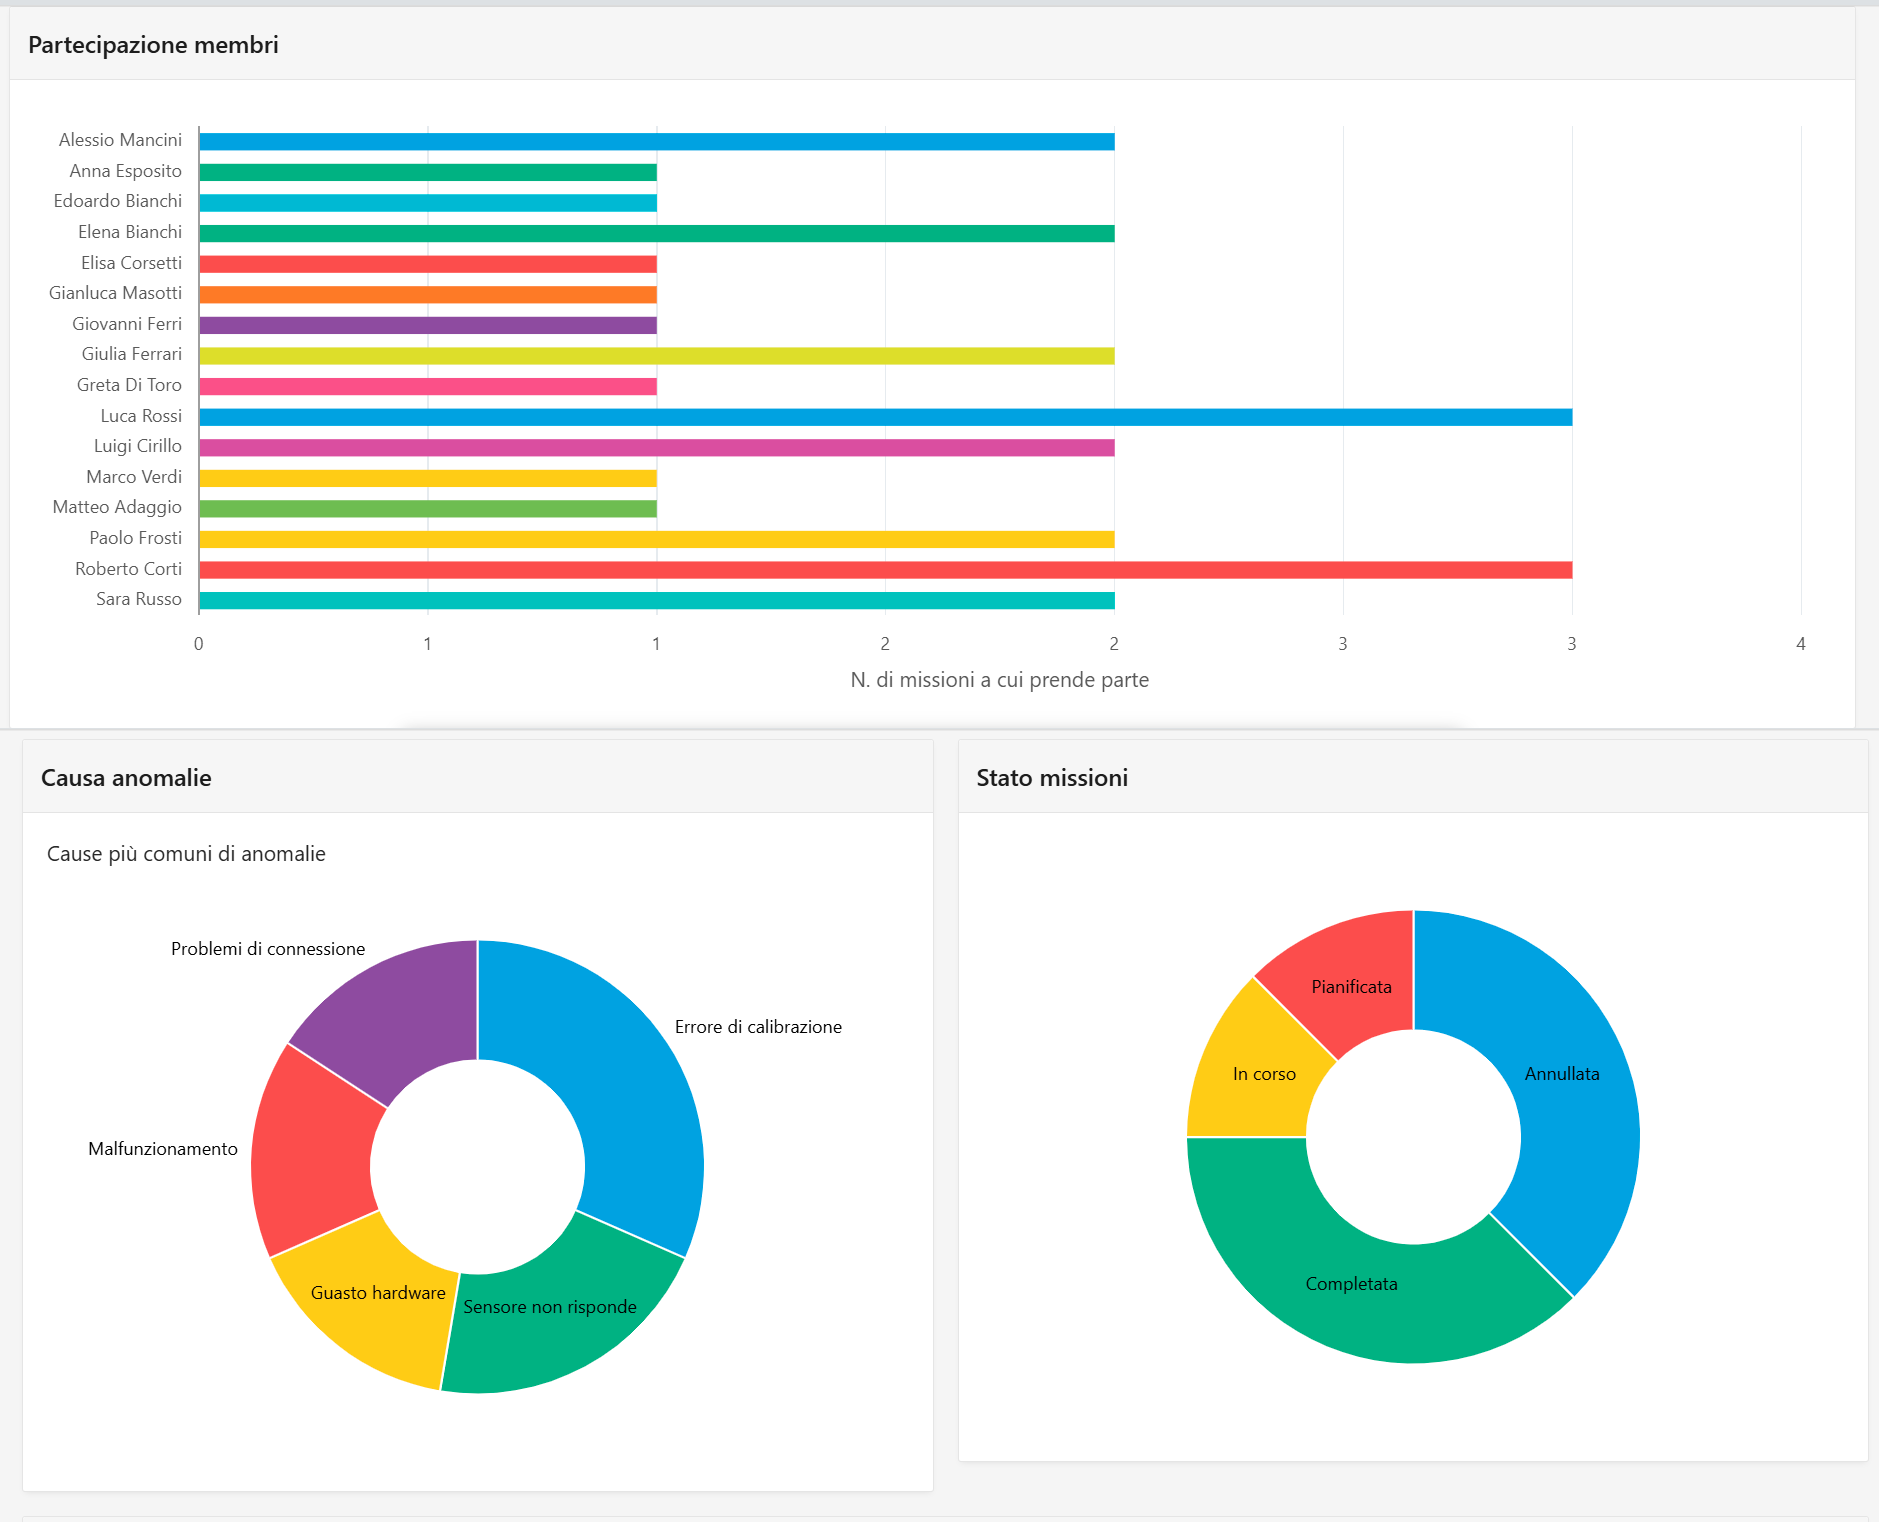
\includegraphics[width=\textwidth]{Media/App/analisi_dati.png}
    \caption{Schermata della sezione \textit{Analisi dati}}
    \label{fig:analisi_dati}
\end{figure}

L'immagine (Figura~\ref{fig:analisi_dati}) mostra la sezione \textbf{Analisi Dati} dell'applicazione ``Missione Lunare'', che fornisce una panoramica visiva sulle principali informazioni relative alla missione. La schermata include diversi grafici, tra cui:

\paragraph*{Partecipazione membri}
Un grafico a barre orizzontali che mostra il numero di missioni a cui ciascun membro del team partecipa. Questo consente di visualizzare rapidamente il grado di coinvolgimento dei membri nelle attività.

\paragraph{Causa anomalie}
Un grafico a ciambella che rappresenta le cause più comuni di anomalie registrate durante le missioni.

\paragraph*{Stato missioni}
Un secondo grafico a ciambella che evidenzia la distribuzione delle missioni in base al loro stato attuale. \\

\noindent
Questa sezione offre una visione chiara e intuitiva per monitorare il progresso e le criticità delle missioni, supportando un processo decisionale informato.


\subsection{Altre views}
Di seguito sono riportate altre sezioni presenti nell'applicazione:
\begin{figure}[ht!]
    \centering
    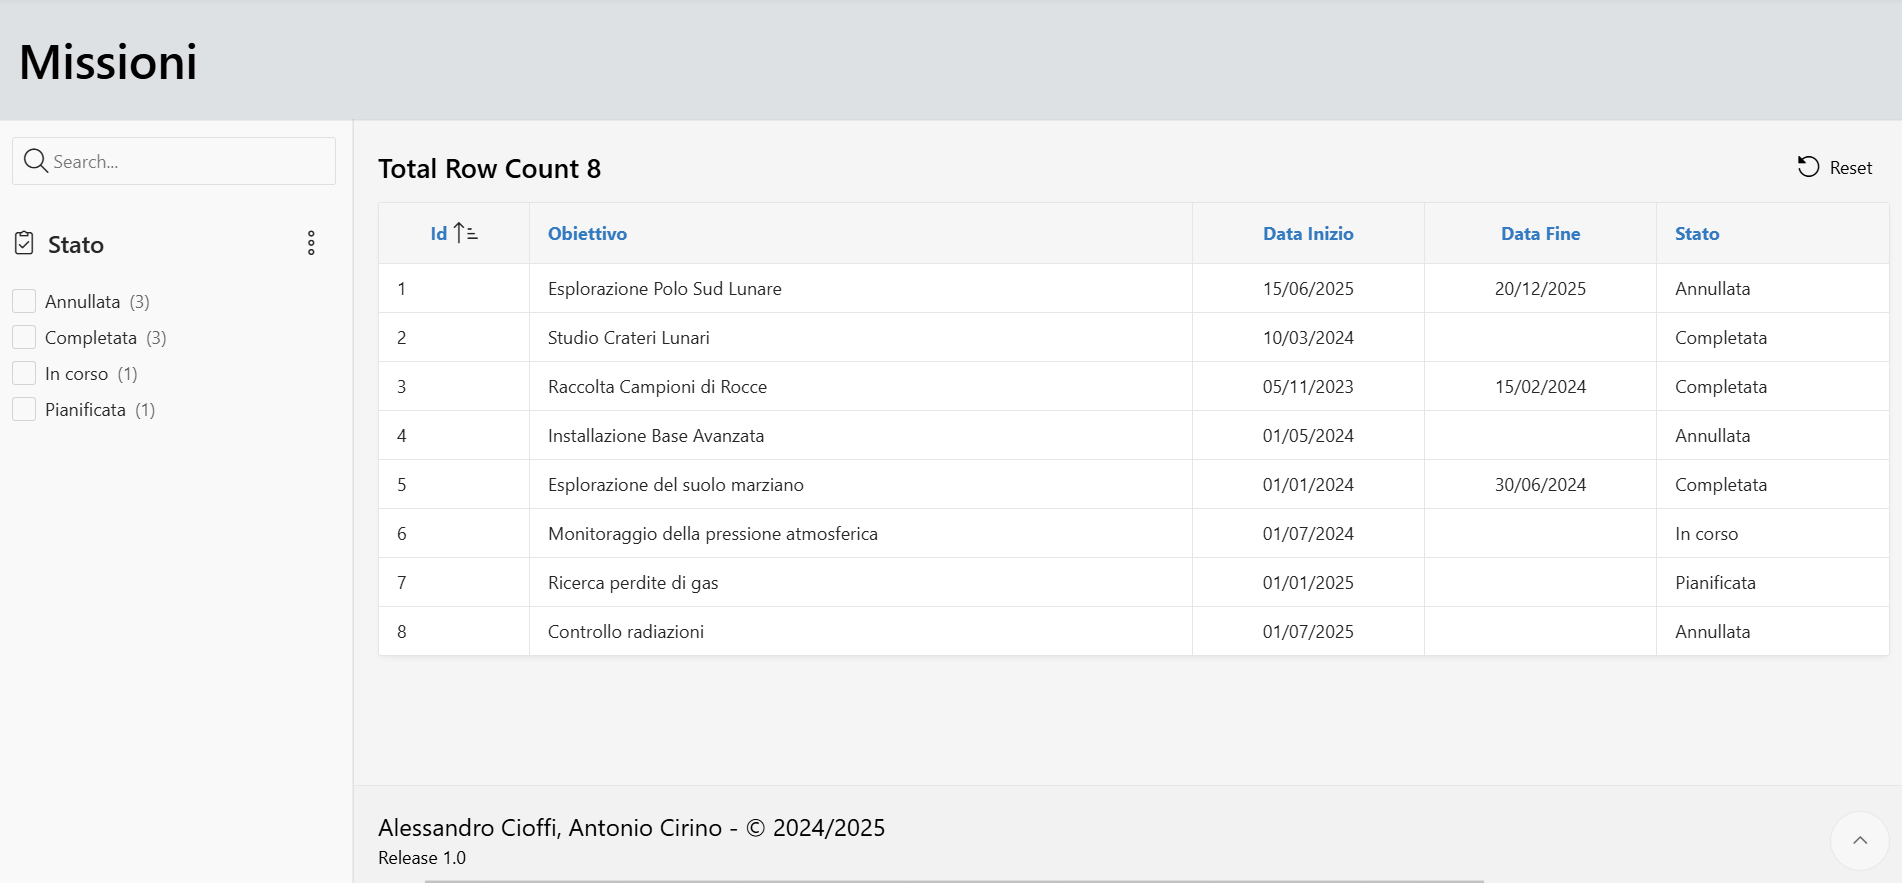
\includegraphics[width=0.9\textwidth]{Media/App/missioni.png}
    \caption{Schermata della sezione \textit{Missioni}}
    \label{fig:missioni}
\end{figure}
\begin{figure}[ht!]
    \centering
    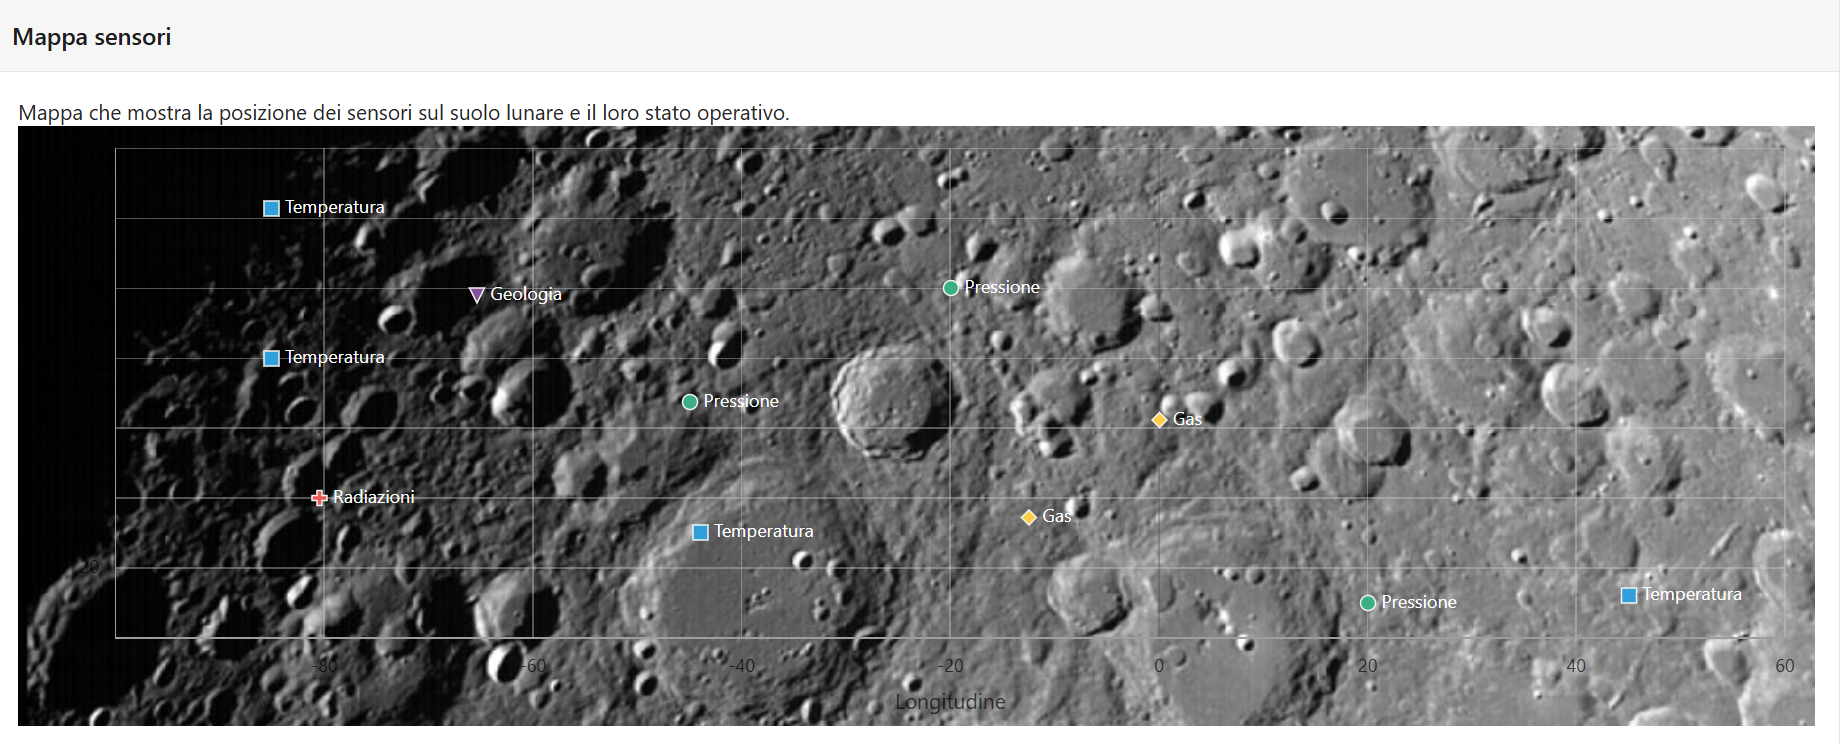
\includegraphics[width=0.9\textwidth]{Media/App/mappa_sensori.png}
    \caption{Schermata della sezione \textit{Mappa}}
    \label{fig:mappa}
\end{figure}
\begin{figure}[ht!]
    \centering
    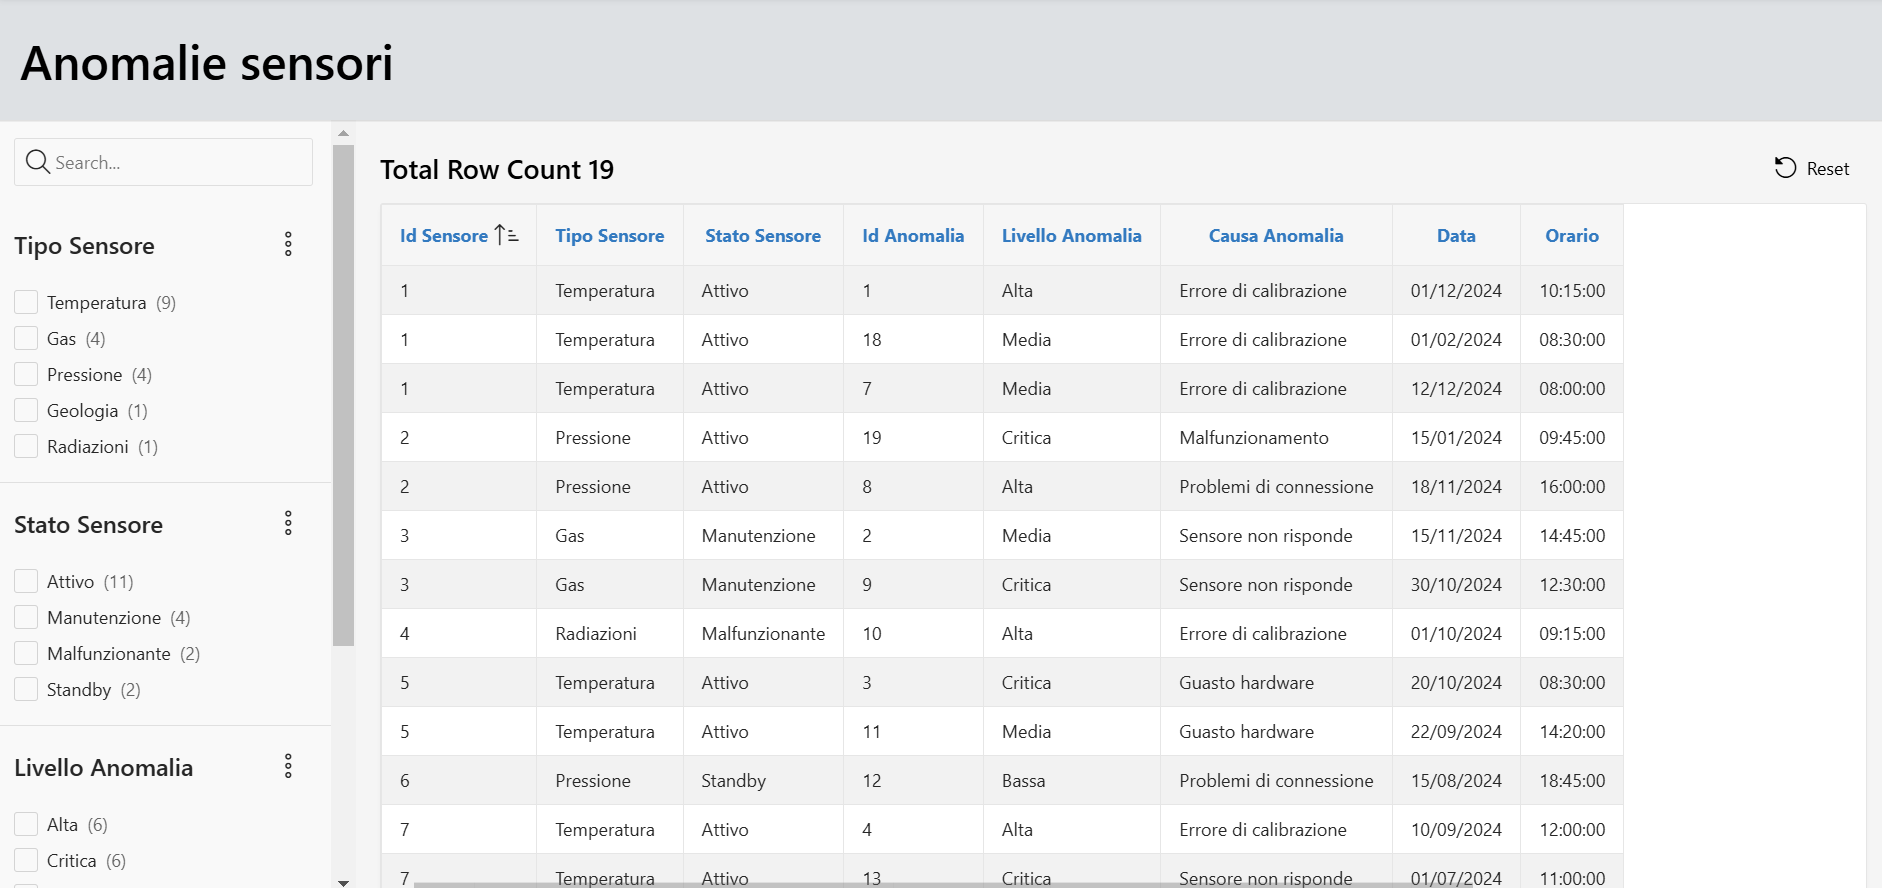
\includegraphics[width=0.9\textwidth]{Media/App/anomalie.png}
    \caption{Schermata della sezione \textit{Anomalie}}
    \label{fig:anomalie}
\end{figure}
\begin{figure}[ht!]
    \centering
    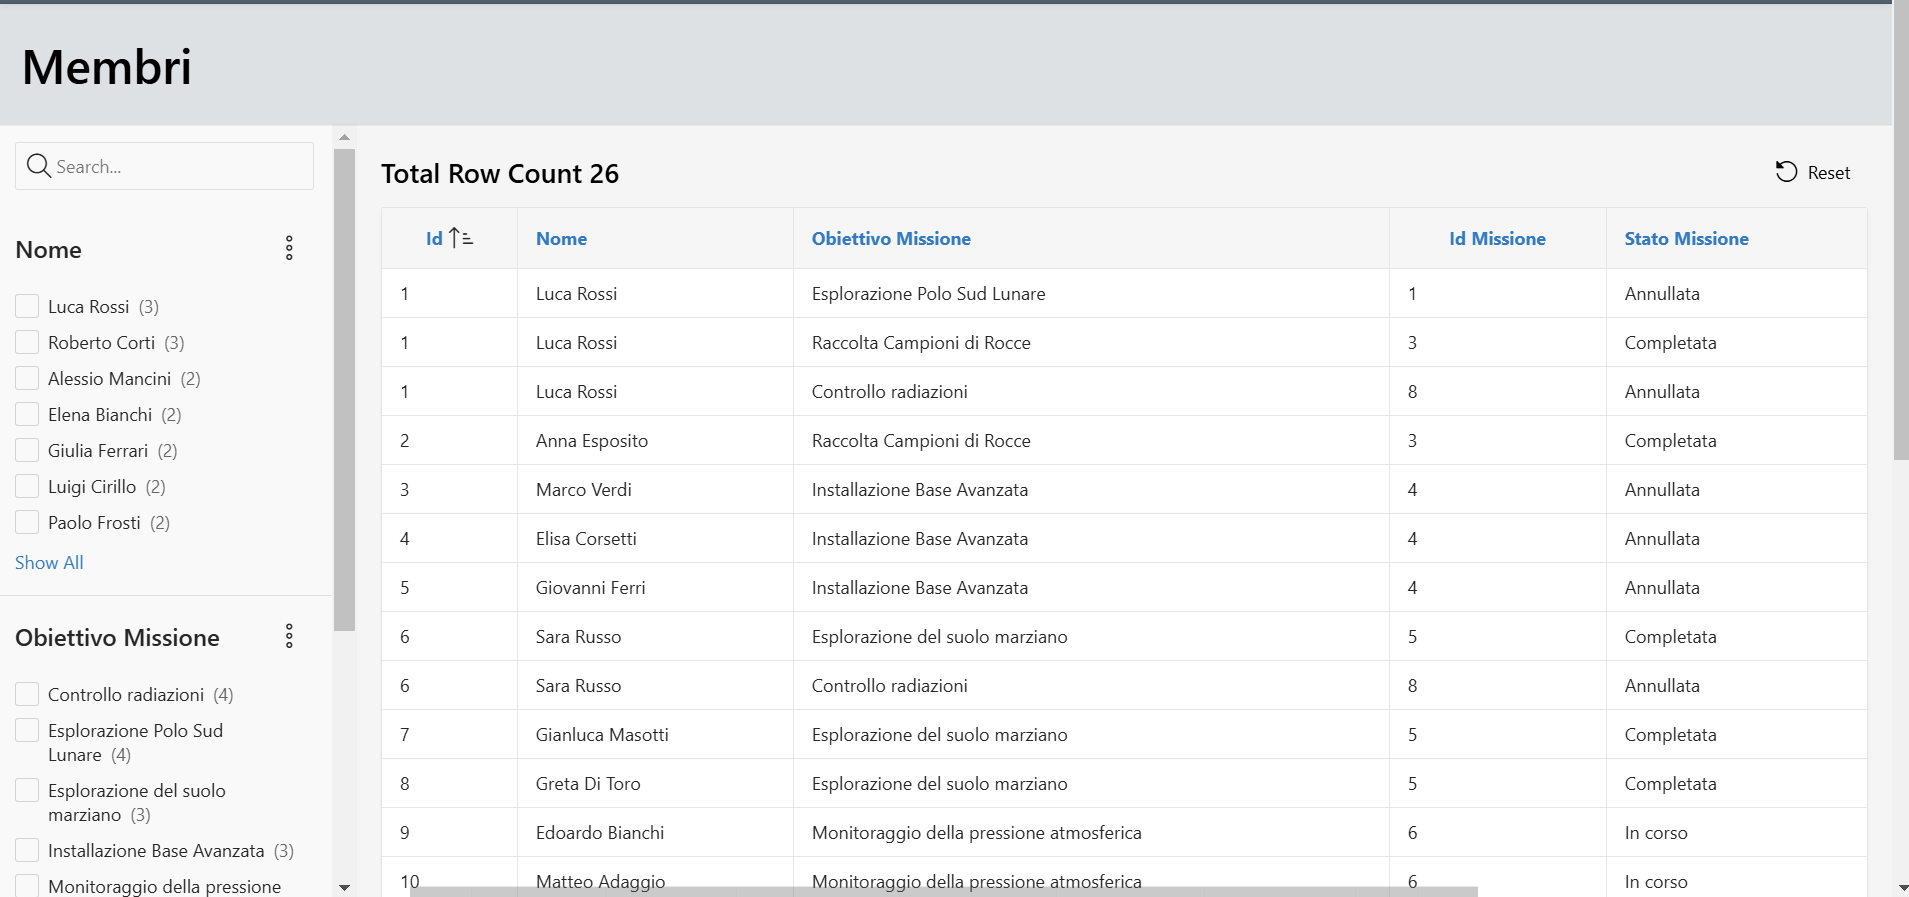
\includegraphics[width=0.9\textwidth]{Media/App/membri.png}
    \caption{Schermata della sezione \textit{Membri}}
    \label{fig:membri}
\end{figure}

\newpage
\subsection{Gestione della sicurezza}
Grazie alla sua profonda integrazione con il database Oracle, APEX garantisce sicurezza, affidabilità e un'elevata scalabilità, rendendolo ideale per progetti di qualsiasi dimensione, dalle piccole imprese alle grandi organizzazioni. \\

\begin{figure}[ht!]
    \centering
    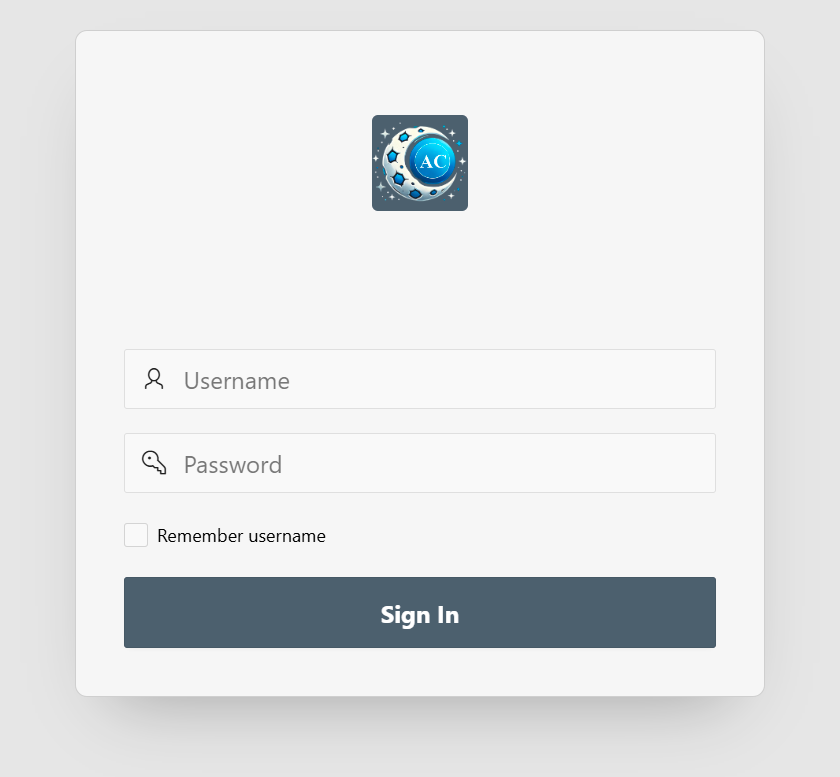
\includegraphics[width=0.5\textwidth]{Media/App/login.png}
    \caption{Schermata di login}
    \label{fig:login}
\end{figure}

\noindent
L'immagine (Figura~\ref{fig:login}) mostra la schermata di login dell'applicazione che implementa le best practice per garantire la sicurezza e la protezione dei dati. Questa schermata rappresenta il primo livello di sicurezza dell'applicazione, garantendo che solo utenti autorizzati possano accedere alle funzionalità e ai dati critici del sistema.
L'accesso all'applicazione è protetto da un sistema di login che richiede l'inserimento di username e password.\\
Oracle APEX utilizza inoltre meccanismi di crittografia per garantire la protezione delle credenziali durante la trasmissione dei dati e il sistema è progettato per prevenire vulnerabilità come SQL injection e brute force.






\end{document}
